\documentclass[12pt]{optlab-bachelor}
\usepackage{amsfonts}
\usepackage{amsmath,amssymb}
\usepackage{algorithm}
\usepackage{algorithmic}
\usepackage[dvipdfmx]{graphicx}

\def\年度{2017}
\def\氏名{天本 祐希}
\def\学生番号{15713004}
\def\題目{並列機械モデルにおける\\最大実行開始待ち時間最小化問題の計算論的分析}
\def\背題目{並列機械モデルにおける最大実行開始待ち時間最小化問題の計算論的分析}

\renewcommand{\bibname}{参考文献}

\begin{document}
\frontmatter

\chapter{はじめに}\label{c_1}
\section{研究背景}
一般に,Webアプリケーションサービスを運用している会社では,運用しているWebアプ
リケーションの応答が遅いと,顧客離れやクレームの被害を受けることがある.
そのため,計算サーバーの応答の早さは重要である.応答の早い計算サーバー
を作るためには,与えられたタスクをどのように割り当て,処理するかを考える必要がある.
計算サーバーのタスクの処理開始は,Webサービスの利用者が,ネットワーク
を介して,そのサービスを運用している会社の計算サーバーにタスクの処理の
要求を行い,そのタスクが計算サーバーに到着した後である.そのため,タス
クの到着時刻とは,タスク処理の処理開始可能時刻である.最大実行開始待ち時間
最小化問題とは,処理開始可能時刻を制約とし,タスクが到着してから,タス
ク処理が開始されるまでの時間,つまり,Webサービス利用者の不満の最小化
を目的とするスケジューリング問題である.

一般に,計算サーバーは,割り当てるタスクの情報があらかじめわからない.つまり,いくつのタスクが,いつ,どの程度処理に時間がかかるのかなどの情報がわからない.計算サーバーはタスクが到着して初めて,そのタスクの処理開始可能時刻がわかる.しかし,そのタスクの処理時間は処理が完了するまでわからない.つまり,タスクをどの計算サーバーに割り当てるかを決定するための指標となるパラメータは処理開始可能時刻のみである.このように,割り当てるタスクの情報があらかじめわからない状況で,スケジュールを決定する問題をオンラインスケジューリング問題という.つまり,計算サーバーへのタスク割り当ては,最大実行開始待ち時間最小化を目的とするオンラインスケジューリング問題として捉えることができる.

オンラインスケジューリング問題では,タスクを割り当てる指標として利用できるパラメータが,処理開始可能時刻のみであるため,タスクが計算サーバーに到着した順で処理するのが自然である.また,本研究の目的関数である最大実行開始待ち時間は,(タスクの処理開始時刻 - タスクの処理開始可能時刻)であるため,オンライン環境では,タスクが到着した順に処理を行うが最善であると言える.

実行開始待ち時間を軸にとったスケジューリング問題の多くは,オフライン環境とオンライン環境のどちらの場合でも未だ研究されていないことが明らかとなった.

\section{研究目的}
最大実行開始待ち時間最小化問題はどの機械モデルにおいても計算複雑さが
明らかでなく,問題の難しさに与える影響の本質は現れていない.
本研究の目的は以下である.
\begin{description}
  \item[目的 1 : ]
  最大実行開始待ち時間最小化問題を定式化し,計算複雑さを明らかにする.

  \item[目的 2 : ]
  同一並列機械モデルにおける最大実行開始待ち時間最小化問題に対するヒューリスティックの開発と解法の評価を行う.

  本研究で提案する解法により求まる解と最適解を比較し提案解法の評価を行う.

  \item[目的 3 : ]
  分枝限定法を改良し,分析対象を拡張する.

  本研究で,無関連並列機械モデルにおける最大実行開始待ち時間最小化問題が NP 完全であることを証明した.
  NP 完全な問題に対する多項式アルゴリズムは存在しないと考えられている.そのため,本研究では,分枝限定法を用いて最適解を求めている.分析対象を拡張するために,分枝限定法に改良を加え,計算効率を向上させる.
\end{description}

\section{研究成果}
本研究では,最大実行開始待ち時間最小化問題に関して以下の成果を得た.
\begin{description}
  \item[成果 1 : ]
  最大実行開始待ち時間最小化問題を決定問題として捉えたとき,無関連並列機械モデルにおいて機械数が入力の一部の場合,NP完全であることを明らかにした.

  最大実行開始待ち時間最小化問題はどの機械モデルにおいても,計算複雑さが明らかではなかった.本研究では,3 SAT からの還元により,無関連並列機械モデルにおいて,機械数が入力の場合,NP 完全であることを証明した.
  \item[成果 2 : ]
  提案解法により求まる解が最適なスケジュールにおける解に近いという結果を得た.

  提案解法により求まる解を $S_g$,最適解を $S_{opt}$ とすると,異なるインスタンスに対して,$S_g/S_{opt}$ を求めることで,提案解法の評価を行った.$S_g/S_{opt}$ の値が 1 に近いほど,解法の質は良いと言える.本研究の実験によると,平均 $S_g/S_{opt} = ?$ の結果を得た.

  \item[成果 3 : ]
  部分問題に対する多項式アルゴリズムの概念を取り入れ,分析対象を拡張した.

  NP 困難な最適化問題は多項式時間で解を求めることができないと考えられている.
  そのため,最適解を求めるためには,実行可能解を全列挙し比較する必要がある.
  そこで,本研究では,分枝限定法に部分問題に対する多項式アルゴリズムの概念を取り入れ,探索する部分木を減らすことで,分析対象の拡張を可能にした.
\end{description}

\section{章構成}
第~\ref{c_2}~章では,最大実行開始待ち時間最小化問題の定式化を行なう.また,既存のスケジューリング問題と対応づけるため,NP完全性の証明のために,最大実行開始待ち時間最小化問題を決定問題として捉えたときの定式化も行なう.

第~\ref{c_3}~章では,本研究で扱う問題に関連する,JITジョブ荷重和最大化問題と
処理開始可能時刻付き最大遅れ時間最小化問題に対する従来研究の成果を,計
算複雑さの観点,解法の観点から,それぞれまとめる.

第~\ref{c_4}~章から第~\ref{c_5}~章にかけて,本研究の成果を述べる.第~\ref{c_4}~章では,まず,無関連並列機械モデルにおける最大実行開始待ち時間最小化問題の計算複雑さに
ついて述べる.

第~\ref{c_5}~章では,提案解法の紹介と,分析対象拡張のために改良した分枝限定法の紹介を行う.また,実験により得たデータから提案解法の評価を行う.

第~\ref{c_6}~章では,結論として,本研究の成果と今後の課題を述べる.

第~\ref{c_7}~章では,第~\ref{c_5}~章で提案した解法の分析に用いた実験結果を載せる.

\chapter{問題の定式化}\label{c_2}
ここでは,最大実行開始待ち時間最小化問題を定式化する.以下 2 つの定式化に共通する,機械モデルについて示す.

各ジョブを処理する機械の性能によって,機械モデルは次のように分類され
る.まず,ジョブを処理する機械の台数について,一つの機械で処理する単一
機械モデルと,複数の機械で処理を行なう並列機械モデルに分類される.並列
機械モデルはさらに,全ての機械の性能が等しい同一並列機械モデル,機械ご
とに処理速度が異なる一様並列機械モデル,ジョブと機械の組み合わせによっ
て処理時間が異なる無関連並列機械モデルに分類される.

\section{最大実行開始待ち時間最小化問題}
最大実行開始待ち時間最小化問題とは,各ジョブの処理開始可能時刻を制約
とし,処理開始可能時刻と処理開始時刻の差の最大値の最小化を目的とするス
ケジューリング問題である.

以下では,無関連並列機械モデルについて,最大実行開始待ち時間最小化問
題を定式化する.
\begin{description}
  \item[入力:] ジョブの集合を $\mathcal{J}$,無関連機械の集合 $\mathcal{M}$と表記し,
  $J \in \mathcal{J}$ を $M \in \mathcal{M}$ で処理する.
  処理開始可能時刻関数 $r : \mathcal{J} \to \mathbb{N}$,処理
  時間関数 $p : \mathcal{J} \times \mathcal{M} \to \mathbb{N}$
  であり,それぞれの関数が返す値は自然数である.入力は2項組,$(p,r)$ と
  表す.
  \item[解:] 問題の前提に基づき,スケジュールを定式化する.スケジュールは以下の条
  件を満たす $A : \mathcal{J} \to \mathcal{M}$ と $s : \mathcal{J} \to
  \mathbb{N}$ の対$(A,s)$ であり,スケジュールによって,各ジョブを,どの
  機械で,いつ処理するかを決める.
  \begin{itemize}
    \item $\forall J \in \mathcal{J}\big[s(J) \ge r(J) \big]$
    \begin{itemize}
      \item 各ジョブは処理開始可能時刻以降に処理を開始する
    \end{itemize}

    \item {\scriptsize $\forall J, J' \in \mathcal{J}\ \Big[ \big[J\neq J' \land A(J) = A(J')\big] \Rightarrow [s(J), s(J)+p(J,A(J))) \cap[s(J'), s(J')+p(J', A(J'))) = \emptyset \Big]$}
    \begin{itemize}
      \item 各機械は同時に複数のジョブを処理しない
      \item 各ジョブの処理を開始すると,完了するまで中断しない
    \end{itemize}
  \end{itemize}

  \item[目的関数:] 実行可能なスケジュール $(A,s)$ のうち,最大の実行開始待ち時間,
  $$\varphi(A,s) = \displaystyle \max_{J \in \mathcal{J}}\{s(J) -
  r(J)\}$$
  を最小とするスケジュールを求める.
\end{description}

\section{最大実行開始待ち時間最小化問題(決定問題)}
最大実行開始待ち時間最小化問題(決定問題)とは,各ジョブの処理開始可能時刻を制約
とし,処理開始可能時刻と処理開始時刻の差の最大値が $w$ 以下となるスケ
ジュールが存在するかを判定する問題である.

以下では,無関連並列機械モデルについて,最大実行開始待ち時間最小化問
題を定式化する.

\begin{description}

  \item[Instance : ] ジョブの集合 $\mathcal{J}$ を無関連機械の集合 $\mathcal{M}$と表記し,
  $J \in \mathcal{J}$ を $M \in \mathcal{M}$ で処理する.
  処理開始可能時刻関数 $r : \mathcal{J} \to \mathbb{N}$,処理
  時間関数 $p : \mathcal{J} \times \mathcal{M} \to \mathbb{N}$,実行開始
  待ち時間 $w$ であり,それぞれの関数が返す値は自然数である.入力は3項組,$(p,r,w)$ と
  表す.

  \item[Question : ] 以下の条件を満たす $A : \mathcal{J} \to \mathcal{M}$ と $s : \mathcal{J} \to \mathbb{N}$ の対$(A,s)$ が存在するかどうか.
  \begin{itemize}
    \item $\forall J \in \mathcal{J}\big[s(J) \ge r(J) \big]$
    \begin{itemize}
      \item 各ジョブは処理開始可能時刻以降に処理を開始する
    \end{itemize}
    \item {\scriptsize $\forall J, J' \in \mathcal{J}\ \Big[ \big[J\ne J' \land A(J) = A(J')\big] \Rightarrow [s(J), s(J)+p(J,A(J))) \cap[s(J'), s(J')+p(J', A(J'))) = \emptyset \Big]$}
    \begin{itemize}
      \item 各機械は同時に複数のジョブを処理しない
      \item 各ジョブの処理を開始すると,完了するまで中断しない
    \end{itemize}
    \item $\max\big\{s(J) - r(J) \mid J \in \mathcal{J}\big\} \le w$
    \begin{itemize}
      \item ジョブの処理開始可能時刻からその処理を開始するまでの待ち時間は $w$ 以下
    \end{itemize}
  \end{itemize}
\end{description}

\subsection{既存のスケジューリング問題との対応}
以下では,最大実行開始待ち時間最小化問題と,JIT ジョブ荷重和最大化問題
と処理開始可能時刻付き最大遅れ時間最小化問題との共通部分と差分をまとめ
る.

\begin{itemize}
  \item \textbf{JIT ジョブ荷重和最大化問題との共通部分}

  実行開始待ち時間 $w$ の制約が最も強い場合,つまり,$w = 0$ のとき,各ジョブは処理開始可能時刻ちょうどで処理を開始しなければならないので,最大実行開始待ち時間最小化問題は JIT ジョブスケジューリング問題として捉えることができる.

  \item \textbf{JIT ジョブ荷重和最大化問題との差分}

  JIT ジョブ荷重和最大化問題では,納期以前に処理を完了したジョブの荷重和
  最大化であるのに対し,最大実行開始待ち時間最小化問題では,全てのジョブ
  の実行開始待ち時間を $w$ 以下にする必要がある.つまり,JIT ジョブ荷重和最大化問題では,目的関数に影響を与えるジョブが全体の一部であることに対し,最大実行開始待ち時間最小化問題では,全てのジョブが影響を与える.

  \item \textbf{処理開始可能時刻付き最大遅れ時間最小化問題との共通部分}

  最大実行開始待ち時間最小化問題(決定問題)は,ジョブが処理開始可能時刻と(処理開始可能時刻 + w)の間で処理可能かという問題に置き換えることができる.さらに,最大遅れ時間最小化問題を最大遅れ時間が $\ell$ 以下となるスケジュールが存在するか,という決定問題に変換したとき,ジョブは処理開始可能時刻と(納期 - 処理時間 - $\ell$)の間で処理可能かという問題に置き換えることができる.このとき,どちらの問題も入力と(入力 + 定数(入力))の間で処理可能かという問題に置き換えることができる.

  \item \textbf{処理開始可能時刻付き最大遅れ時間最小化問題との差分}

  処理開始可能時刻付き最大遅れ時間最小化問題では,処理開始可能時刻と納期の間で処理可能かという問題として捉えることができる.このとき,納期 = 処理開始可能時刻 + 処理時間 と納期により制限を加えた問題が,最大実行開始待ち時間最小化問題に対応する.
  つまり,処理開始可能時刻付き最大遅れ時間最小化問題は最大実行開始待ち時間最小化問題の拡張問題として捉えることができる.

\end{itemize}

以上の点から,次の章では,JIT ジョブ荷重和最大化問題
と処理開始可能時刻付き最大遅れ時間最小化問題の従来研究の成果を紹介する.

\chapter{従来研究}\label{c_3}
ここでは,JITジョブ荷重和最大化問題と,処理開始可能時刻付き最大遅れ
時間最小化問題について,従来研究の成果を紹介する.

\section{JITジョブ荷重和最大化問題}
この問題は 3-SAT からの還元により,強 NP 困難であることが Sung, S. C., and Vlach(2005) \cite{JIT}
によって証明されている.以下では,JIT ジョブ荷重和最大化問題を定式化し,その後,3-SAT の定義を踏まえ問題が NP 困難であることの証明を示す.証明の記述は 川俣友佳(2012)\cite{kawamata}
を参考にした.
\subsection{定式化}
\begin{description}
  \item[入力:] $n$ 個のジョブ $J_1,\ldots,J_n$ を $m$ 台の同一機械 $M_1,\ldots,M_m$
  で処理する.入力は,各ジョブ $J_i ( i \in \{1,\ldots,n\} )$ の,処理時
  間 $p_i$ ,処理開始可能時刻 $r_i$ ,納期 $d_i$ ,荷重 $w_i$ であり,
  それぞれの値は自然数である.
  各ジョブの処理時間をまとめて $P = (p_1,\ldots,p_n) \in \mathbb{N}^n$,
  処理開始可能時刻をまとめて $R = (r_1,\ldots,r_n) \in \mathbb{N}^n$ ,
  納期をまとめて $D = (d_1,\ldots,d_n) \in \mathbb{N}^n$ ,
  荷重をまとめて $W = (w_1,\ldots,w_n) \in \mathbb{N}^n$ と表し,
  入力 は 4 項組,$(P,R,D,W)$ と表す.
  \item[解:] 問題の前提に基づき,スケジュールを定式化する.スケジュールは以下
  の条件を満たす $\forall j \in \{1,\ldots,m\}\big[A_j \subseteq
  \{1,\ldots,n\}\big]$ と $C : \{1,\ldots,n\} \to \mathbb{N}$ の対 $(A,
  C)$ であり,スケジュールによって,各ジョブを,どの機械で,いつ処理をするかを決める.
  \begin{itemize}
    \item {\small $\forall i, i' \in \{1,\ldots,n\}\ \Big[ \big[i \neq i' \land A_i = A_{i'}\big] \Rightarrow [C(i) - p_j, C(i)) \cap [C(i') - p_{i'}, C(i')) = \emptyset \Big]$}
    \item  $\forall i \in \{1,\ldots,n\}\big[C(i) - p_i \ge r_i\big]$
  \end{itemize}
  \item[目的関数:] 実行可能なスケジュール $(A, C)$ のうち,納期以前に処理を完了するジョ
  ブの荷重和,
  $$\displaystyle \varphi(A,C) = \sum_{i \in \mathcal{Q}(A,C)}w_i$$,
  $i \in \mathcal{Q}(A,C)$ を最大とするスケジュールを求める.ただし,
  $\mathcal{Q}(A, C)$ はスケジュール $(A, C)$ に
  おいて納期以前に処理を完了するジョブの集合である (
  $\mathcal{Q}(A, C) = \{i \in \{1,\ldots, n\} | C(i) \ge d_i \}$ ).
\end{description}

\subsection{計算複雑さの証明}
3 SAT からの還元により,JIT ジョブ荷重和最大化問題の計算複雑さの証明を行う.
3 SAT の定義は以下である.
\begin{description}
  \item[Instance : ] ブール型の変数集合 $X$ と,$X$ 上の 3 つのリテラル
  からなる集合の集合 $H$ (各 $h \in H$ は $|h| = 3$ を満たす).
  \item[Question : ] $H$ を充足する真理値割り当て $f ; X \to \{0,1\}$,
  つまり,
  $$\displaystyle \bigwedge_{h \in H} \bigg(\bigvee_{x \in h}f(x) \lor
  \bigvee_{\bar x \in h}\lnot f(x) \bigg) = 1$$
  を満たす $f$ が存在するか?
\end{description}

ブール型変数の集合 $X = \{x_1,\ldots,,x_β\}$ と, $X$ 上の 3 つのリテラル
からなる集合 $H = {h_1,\ldots,h_{\lambda}}$ の 2 項組, $(X,H)$ を任意の
3-SAT 問題の入力とする.
議論に先立ち,いくつかの表記を導入する.各 $k \in \{1,\ldots,\beta\}$
について, $\gamma_k$ を $H$ に おいて $x_k$ が現れる回数を表す自然
数とし, $\gamma$ を $\gamma_k ( k \in \{1,\ldots,\beta\} )$の最大値に
1 を加えた値とする($\displaystyle \gamma = \max_{k \in \{1,2,\ldots, \beta\}} \{\gamma_k \}+ 1$).
$(X, H)$ に基づき,以下のように JIT ジョブ荷重和最大化問題の入力
を設定する. $2\beta_{\gamma}$ 個のジョブを $\lambda + \beta$ 台の
無関連機械で処理する.各ジョブの処理時間,納期ズレ幅,納期,荷
重を以下のように設定する.

\begin{description}
  \item[納期ズレ幅の設定:]
  各ジョブ $i \in \{1,\ldots,2\beta \gamma\}$ の納期ズレ幅
  $\alpha_i$ を 0 とする.
  \item[納期の設定:] $\{1,2,\ldots, \beta \gamma\}$$ の $$\beta \gamma$ 個ジョブの納期につ
  いて,昇順で $\gamma$ 個ずつとった $\beta$ 個のグループについて,機械
  を順に対応させる.
  各グループ $k \in \{1,2,\ldots, \beta\}$ の $\gamma$ 番目のジョブの納
  期を $2\gamma - 1$,$\ell$ 番目のジョブ ( $\ell \neq \gamma$ ) の納期
  を $\ell$ とする.つまり,各 $k \in \{1,2,\ldots, \beta\}$ と $\ell \in \{1,2,\ldots,
  \gamma\}$について,
  $$d_{(k - 1)\gamma + \ell} = \left\{ \begin{array}{ll} \ell & \text{if } \ell < \gamma \\ 2\gamma - 1 & \text{if } \ell = \gamma \end{array} \right.$$
  $\{\beta \gamma + 1,\ldots, 2\beta \gamma\}$ の $\beta \gamma$ 個のジョ
  ブの納期についても,同様に対応させる.
  各グループ $k \in \{1,2,\ldots, \beta\}$ の $\gamma$ 番目のジョブの納期を $\gamma$,$\ell$ 番目のジョブ ( $\ell \neq \gamma$ ) の納期を $\gamma + \ell$ とする.
  つまり,各 $k \in \{1,2,\ldots, \beta\}$ と $\ell \in \{1,2,\ldots,
  \gamma\}$について,
  $$d_{(\beta + k - 1)\gamma + \ell} = \left\{ \begin{array}{ll}\gamma +  \ell & \text{if } \ell < \gamma \\ \gamma & \text{if } \ell = \gamma \end{array} \right.$$
  \item[荷重和の設定:] 各ジョブを納期昇順に基づき $2\beta$ 個のグループに分ける.
  グループ $k \in \{1,2,\ldots,\beta\}$ と,グループ $k + \beta$ について,グループの $\gamma$ 番目のジョブの荷重を $\gamma$ とし,それ以外のジョブの荷重を 1 とする.
  つまり,各 $k \in \{1,2,\ldots, \beta\}$ と $\ell \in \{1,2,\ldots,
  \gamma\}$について,
  $$w_{(k - 1)\gamma + \ell^v} = w_{(\beta + k - 1)\gamma + \ell} = \left\{ \begin{array}{ll} 1 & \text{if } \ell < \gamma \\ \gamma & \text{if } \ell = \gamma \end{array} \right.$$
  \item[処理時間の設定:] 各ジョブを納期昇順に基づき $2\beta$ 個のグループに分ける
  グループ $k \in \{1,2,\ldots,\beta\}$ に機械を $k$ に対応させ,グルー
  プ $k + \beta$ にも同様に機械 $k$ を対応させる.各グループの各ジョブについて, グループに対応した機械以外の各機械における処理時間を $2\gamma$ とする.
  各グループの $\gamma$ 番目のジョブの,グループに対応する機械における処
  理時間を $\gamma$ とし,$\gamma$ 番目のジョブをのぞいた各ジョブの,グループに対応する機械における処理時間を 1 とする.
  つまり,各 $j \in \{1,2,\ldots, \beta\}$ と $k \in \{1,2,\ldots,
  \beta\}$ と $\ell \in \{1,2,\ldots, \gamma\}$について,
  $$p_{(k - 1)\gamma + \ell, j} = p_{(\beta + k - 1)\gamma + \ell, j} = \left\{ \begin{array}{ll} 1 & \text{if } \ell < \gamma \text{ and } j = k, \\ \gamma & \text{if } \ell = \gamma \text{ and } j = k, \\ 2\gamma & \text{otherwise}\end{array} \right.$$

  残りの各機械 $j \in \{\beta + 1, \ldots , \beta + \gamma\}$ について,各ジョブの処理時間を設定する
  各グループ $k \in \{1,2,\ldots,\beta\}$ について,$x_k$ を対応させる.
  各グループ $k \in \{1,2,\ldots,\beta\}$ について,$\ell \in \{1,2,\ldots, \gamma - 1\}$ 番目の各ジョブにつ いて,$x_k \in h_{j - \beta}$ であれば $d_{(k - 1)\gamma + 1}$ とし,そうでない場合は $2\gamma$ とする.また,$\gamma$ 番目 のジョブの処理時間は $2\gamma$ とする.
  グループ $k + \beta$ について$\bar x_k$ を対応させる.
  $\ell \in \{1,2,\ldots, \gamma - 1\}$ 番目の各ジョブについて,$\bar x_k \in h_{j - \beta}$ であれば $d_{(\beta + k - 1)\gamma + \ell}$ とし, そうでない場合は $2\gamma$ とする.また,$\gamma$ 番目のジョブの処理時間は $2\gamma$ とする.
  つまり,各 $j \in \{\beta + 1,\ldots, \beta + \gamma\}$ と $k \in
  \{1,2,\ldots, \beta\}$ と $\ell \in \{1,2,\ldots, \gamma\}$について,
  $$p_{(k - 1)\gamma + \ell, j} = \left\{ \begin{array}{ll} d_{(k - 1)\gamma + 1} & \text{if } \ell < \gamma \text{ and } x_k \in h_{j - \beta}, \\ 2\gamma & \text{otherwise} \end{array} \right.$$

  $$p_{(\beta + k - 1)\gamma + \ell, j} = \left\{ \begin{array}{ll} d_{(\beta + k - 1)\gamma + \ell} & \text{if } \ell < \gamma \text{ and } \bar x_k \in h_{j - \beta}, \\ 2\gamma & \text{otherwise} \end{array} \right.$$
\end{description}

このように設定した $(P,a,D,W)$ は JIT ジョブ荷重和最大化問題の入力である.以降,$(X,H)$ に基づいて前述のように設定した $(P,a,D,W)$ を区別して $I_{(X,H)}$ と表す $(I_{(X,H)} = (P,a,D,W))$.
以下,$H$ を充足する真理値割り当て $f : X \to \{0,1\}$ が存在すること
と,$I_{(X,H)}$ を入力とする JIT ジョブ荷重和最大化問題に対して
$\varphi(A,C) \ge \beta(2\gamma - 1) + \lambda$ を満たす実行可能なスケ
ジュール $(A,C)$ が存在することが,同値であることを示す.

\begin{lemma}\label{l_1}
  $H$ を充足する真理値割り当て $f : X \to \{0,1\}$ が存在するならば,$I_{(X,H)}$ を入力とする JIT ジョブ荷重和最大化問題に対して
  $\varphi(A, C) \ge \beta(2\gamma - 1) + \lambda$ を満たす実行可能なス
  ケジュール $(A, C)$ が存在する.
\end{lemma}

\begin{proof}
  $(X,H)$ を任意の 3 -SAT 問題の入力とし, $f : X \to \{0,1\}$ を $H$ を
  充足する真理値割り当てとする.つまり, $f$ は以下を満たす.
  $$\displaystyle \bigwedge_{h \in H} \bigg(\bigvee_{x \in h}f(x) \lor
  \bigvee_{\bar x \in h}\lnot f(x) \bigg) = 1$$
  各 $k \in \{1,\ldots, \beta\}$ について, $f(x_k) = 1$ ならばグルー
  プ $\beta + k$ の全てのジョブを,グループ $\beta + k$ に対応する機械
  $k$ に割り当て,そうでなければグルー
  プ $k$ の全てのジョ ブを,グループ $k$ に対応する機械 $k$ に割り当てる.ま
  た,機械 $k$ に割り当てた各ジョ ブの完了時刻を納期とする.つまり,
  $f(x_k) = 1$ ならば,各 $\ell \in \{1,\ldots,\gamma\}$ について $A_k
  :=A_k cup\{(\beta+k−1)\gamma+\ell\}$ かつ
  $C((\beta+k−1)\gamma+\ell)=d(\beta+k−1)\gamma+l$ ,$f(x_k)=0$ なら
  ば,各 $\ell \in \{1,\ldots,\gamma \}$ について$A_k :=A_k \cup
  \{(k−1)\gamma+\ell \}$ かつ $C((k−1)\gamma+\ell)=d(k−1)\gamma+\ell$
  . $I_{(X,H)}$ の定義より,ここまでのスケジュールにおいて,機械
  $1,\ldots, \beta$ に割り当てたジョ ブの処理時間は重複せず (図 A.1),完
  了時刻は納期であることから,$k \in \{1,\ldots,\beta\}$ に割り当てたジョ
  ブは JIT ジョブである.よって,ここまでのスケジュール $(A, C)$ における
  JIT ジョブの荷重和は,
  $$\displaystyle \varphi(A,C) = \sum_{k \in
  \{1,\ldots,\beta\}}\bigg(\sum_{i \in \mathcal{Q}(A,C):i \in
  A_k}w_i\bigg) = \sum_{k \in \{1,\ldots,\beta\}}(2\gamma - 1) =
  \beta(2\gamma - 1)$$.
  \begin{center}
    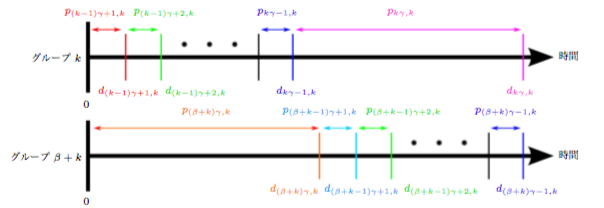
\includegraphics[width = 15cm]{SJIT1.png} \\
    図 $A.1$ : 機械 $k \in \{1,\ldots,\beta\}$ に対応するグループ $k$
    とグループ $\beta + k$ の各ジョブ
  \end{center}
  各 $j\in \{1,\ldots,\lambda\}$ について,$f(x_k)=1$ を満たす$x_k \in
  h_j$ か,$f(x_k)=0$ を満たす $\bar x_k \in h_j$ をひとつ見つける. $f$ が $H$ を充足することから,各 $j \in \{1,\ldots,\lambda\}$ について, 上記を満たすリテラルは必ず存在する.
  与えられた $j \in \{1,\ldots,\lambda \}$ について, $f(x_k) = 1$ を満
  たす $x_k \in h_j$ を見つけたと仮定す る.グループ $k$ のジョブ
  のうち,いずれの機械にも割り当てられていない $\ell \in
  \{1,\ldots,\gamma - 1\}$ を見つける.グループ $k$ のジョブは,
  $f (x_k) = 1$ であることから,$\{1,\ldots, \beta \}$ のいずれの機
  械にも割り当てられておらず,また,各リテラルが現れる回数は高々
  $\gamma − 1$ であることから,そのような $\ell$ 番目のジョブは必す
  ゙存在する. $A_{j + \beta} := A_{j + \beta} \cup \{ (k − 1) \gamma +
  \ell\}$ とし, $C((k − 1)\gamma + l) = d(k−1)\gamma + \ell$ とする.
  次に,与えられた $j \in \{1,\ldots,\lambda\}$ について, $f(x_k) = 0$
  を満たす $\bar x_k \in h_j$ を見つけたと仮定する.グループ $\beta
  + k$ のジョブのうち,いずれの機械にも割り当てられていない $\ell
  \in \{1,\ldots,\gamma\}$ を見つける.先ほどと同様の議論で,そのよ
  うな $\ell$ は必ず存在する. $A_{j + \beta} := A_{j + \beta} \cup \{
  (\beta + k − 1 ) \gamma + \ell \} = j + \beta$ とし,$C((\beta + k −
  1) \gamma + \ell) = d(\beta + k − 1)\gamma + \ell$ とする.
  各グループの $\ell \in \{1,\ldots,\gamma − 1\}$ 番目のジョブ
  の荷重が 1 であることから,各 $j \in \{1,\ldots, \lambda \}$ につ
  いて $j$ に割り当てられた JIT ジョブの荷重和は,
  $$\displaystyle \sum_{i \in \mathcal{Q}(A,C):A(i) = j + \beta}w_i =
  1$$
  ここまでのスケジュール $(A, C)$ においていずれの機械にも割り当てられて
  いないジョブを, $\max\{d_i | i \in \{1,\ldots, 2\beta \gamma\}$ のあと,任意の順,任意の機械で処理するものとする.
  明らかにスケジュール $(A, C)$ は実行可能であり,以下を満たす.
  $$\displaystyle \varphi(A,C) = \sum_{j \in
  \{1,\ldots,\beta\}} \sum_{i \in \mathcal{Q}(A,C):i \in
  A_j}w_i + \sum_{j \in
  \{\beta + 1,\ldots,\lambda + \beta\}} \sum_{i \in \mathcal{Q}(A,C):i \in
  A_j}w_i =
  \beta(2\gamma - 1) + \lambda$$.
\end{proof}

ここで, $I_{(X,H)}$ を入力とする JIT ジョブ荷重和最大化問題に
おける実行可能なスケジュールについて,いくつかの性質を示す.
$(A, C)$ を $_{I(X,H)}$ を入力とする JIT ジョブ荷重和最大化問題に
おける任意の実行可能なスケジュールとする.実行可能性の制約により,各シ
゙ョブは機械の稼働開始時刻以降に処理を開始することから,各 JIT ジョ
ブ $i \in \mathcal{Q}(A,C)$ について,$C(i) − p_i = d_i − p_i \ge 0$ であ
る.このことから,$p_i,j \ge 2\gamma$ かつ $d_i \le 2\gamma − 1$ を満
たす $i \in \{1,\ldots,n\}$ と $j \in \{1,\ldots,m\}$ について,$i \in
\mathcal{Q}(A,C)$ のとき,$i \notin A_j$ である.したがって,
$I_{(X,H)}$ の定義より,各 $k \in \{1,\ldots,\beta\}$ について,
\begin{itemize}
  \item $i \in \mathcal{Q}(A,C)$ かつ $i \in A_k$ ならば,
  $(k − 1)\gamma + 1 \le i \le k\gamma$ または $(\beta + k − 1)\gamma +
  1 \le i \le (\beta + k)\gamma$ である.
  \item $k\gamma \in \mathcal{Q}(A,C)$ ならば $k\gamma \in A_k$ であ
  り,$\beta + k)\gamma \in \mathcal{Q}(A,C)$ な
  らば $(\beta + k)\gamma \in A_k$ である.
\end{itemize}
実行可能性の制約より,同じ機械に割り当てられた複数のジョブの処理
は重複しないこと から,各 $k \in \{1,\ldots,\beta\}$ について,
\begin{itemize}
  \item $k\gamma \in \mathcal{Q}(A,C)$ ならば,$i \in A_k$ である任
  意の $i \in \mathcal{Q}(A,C)$ について,$i$ は \\$(k − 1)\gamma− 1
  \le k\gamma$ を満たす (図 $A.1$).
  \item $(\beta + k)\gamma \in \mathcal{Q}(A,C)$ ならば,$i \in A_k$ て
  ゙ある任意の $i \in \mathcal{Q}(A,C)$ について,$i$ は
  $(\beta + k − 1)\gamma − 1 \le i \le (\beta + k)\gamma$ を満たす.
\end{itemize}
以上の議論より,各 $k \in \{1,\ldots, \beta \}$ について,$k$ に割り当
てられた JIT ジョブの荷重和は以下を満たし
\begin{equation}
  \sum_{i \in \mathcal{Q}(A,C):i \in A_k}w_i \le
  2\gamma - 1 \tag{A.1}
\end{equation}

% タグづけがまだできていない
以下のいずれかを満たす場合にのみ,$\displaystyle \sum_{i \in \mathcal{Q}(A,C):i \in A_k}w_i = 2\gamma - 1$ となる.
\begin{equation}
  \{i \in \mathcal{Q}(A,C) \mid i \in A_k\} = \{(k - 1)\gamma + 1, (k
  - 1)\gamma + 2,\ldots,k\gamma\} \tag{A.2}
\end{equation}
\begin{equation}
  \{i \in \mathcal{Q}(A,C) \mid i \in A_k\} = \{(\beta + k -
  1)\gamma + 1, (\beta + k
  - 1)\gamma + 2,\ldots,(\beta + k)\gamma\} \tag{A.3}
\end{equation}
さらに,各 $j \in \{\beta + 1,\ldots, \beta + \lambda \}$ について,
各ジョブ $i \in \{1,\ldots, 2\beta \gamma \}$ の処理時間は $p_ij
\in \{d_i, 2\gamma \}$ であり,機械 $j$ に割り当てられるジョブは
高々 1 つである ( $|\{i \in \mathcal{Q}(A, C)\} | i \in A_j \}| \le 1$
).既に述べたように,各 $k \in \{1,\ldots,\beta \}$ について
$k\gamma \in \mathcal{Q}(A,C)$ ならば $k\gamma \in A_k$ であり,
$(\beta + k) \gamma \in \mathcal{Q}(A,C)$ ならば,$(\beta +
k)\gamma \in A_k$ である.これらのジョブをのぞいた各ジョブの荷
重は 1 であることから,各 $j \in \{ \beta + 1,\ldots,
\lambda + \beta \}$ について,
\begin{equation}
  \displaystyle \sum_{i \in \mathcal{Q}:i \in A_j}w_i \le 1 \tag{A.4}
\end{equation}

\begin{lemma}\label{l_2}
  $I_{(X,H)}$ を入力とする JIT ジョブ荷重和最大化問題に対して
  $\varphi(A, C) \ge \beta(2\gamma − 1) + \lambda$ を満たす実行可能なス
  ケジュール $(A, C)$ が存在するならば,$H$ を充足する真理値割り当
  て $f : X \to \{0, 1\}$ が存在する.
\end{lemma}

\begin{proof}
  $(A, C)$ を $I_{(X,H)}$ を入力とする JIT ジョブ荷重和最大化問題に
  対して $\varphi(A, C) \ge \beta (2\gamma − 1) + \lambda$ を満たす実行
  可能なスケジュールとする.式 ($15$) と式 ($A.4$) より $\varphi(A, C
  )\le≤ \beta(2\gamma − 1) + \lambda$ であり,このことから,
  $\varphi(A, C) = \beta (2\gamma − 1) + \lambda$ である.
  各機械 $k \in \{1,\ldots, \beta\}$ について,式 ($A.2$) または式
  ($A.3$) が満たされ,各 $j \in \{ \beta + 1,\ldots,\beta + \lambda
  \}$ について,$|\{ i \in \mathcal{Q}(A,C) | i \in A_j \} | = 1$ で
  ある.$(A,C)$ に基づき,$f : H \to \{0,1\}$ を以下のように設定する.
  各 $k \in \{1,\ldots, \beta \}$ について,式 ($A.3$) が満たされる
  ならば $f(x_k) = 1$ とし,そうでなければ $f(x_k) = 0$ とする.
  明らかに,各 $j \in \{\beta + 1,\ldots,\beta + \lambda \}$ について
  $j$ に割り当てられたただ一つの JIT ジョブ $i \in
  \mathcal{Q}(A,C)$ が存在し,$i \ge \beta \gamma$ ならば $f(x_k)
  = 1$ を満たすある $x_k \in h_{j - \beta}$ が存在し,$i > \beta
  \gamma$ ならば $f(x_k) = 0$ を満たすある $\bar x_k \in h_{j -
  \beta}$ が存在する.したがって,$f$ は $H$ を充足する真理値割り当てである.
\end{proof}

補題 \ref{l_1} と補題 \ref{l_2} より,$H$ を充足する真理値割り当て $f : X \to \{0,
1\}$ が存在することと,$I_{(X,H)}$ を入力とする JIT ジョブ荷重和
最大化問題に対して $\varphi(A, C) \ge \beta(2\gamma − 1) + \lambda$
を満たす実行可能なスケジュール $(A, C)$ が存在することは,同値で
ある.
3 -SAT 問題の入力 $(X,H)$ に基づく $I_{(X,H)}$ の生成に要する計算時
間は,明らかに多項式時間であり,入力 $I_{(X,H)}$ の長さは,$(X, H)$
の長さに関する多項式で表すことができる.したがって,無関連並列
機械モデルにおいて機械数が入力の一部の場合, JIT ジョブ荷重和
最大化問題は強 NP 困難である.

\section{処理開始可能時刻付き最大遅れ時間最小化問題} %生産管理1
% Chapter3

この問題は 3-PARTITION からの還元により,強 NP 困難であることが証明さ
れている.(Michael L. Pinedo(2016) \cite{Lmax})
以下では,処理開始可能時刻付き最大遅れ時間最小化問題を定式化し,その後,3-PARTITION の定義を踏まえ問題が NP 困難であることの証明を示す.
\subsection{定式化}
\begin{description}
  \item[入力:] $n$ 個のジョブ $J_1,\ldots,J_n$ を 1 台の機械で処理する.入力は,各ジョブ $J_i ( i \in \{1,\ldots,n\} )$ の,処理時間 $p_i$,処理開始可能時刻
  $r_i$,納期 $d_i$ であり,それぞれの値は自然数である.各ジョブの処理時間をまとめて $P =
  (p_1,\ldots,p_n) \in \mathbb{N}^n$ ,処理開始可能時刻をまとめて $R =
  (r_1,\ldots,r_n) \in \mathbb{N}^n$ ,納期をまとめて $D =
  (d_1,\ldots,d_n) \in \mathbb{N}^n$ と表し,入力は 3項組 $(P,R,D)$ と表
  す.
  \item[解:] 問題の前提に基づき,スケジュールを定式化する.スケジュールは以下
  の条件を満たす $C : \{1,\ldots,n\} \to \mathbb{N}$ であり,スケジュー
  ルによって,各ジョブ,をいつ処理をするかを決める.
  \begin{itemize}
    \item $\forall i, i' \in \{1,\ldots,n\}\ \Big[ \big[i \neq i' \big] \Rightarrow [C(i) - p_i, C(i)) \cap [C(i') - p_{i'}, C(i')) = \emptyset \Big]$
    \begin{itemize}
      \item 機械は同時に複数のジョブを処理しない
      \item 各ジョブの処理を開始すると,完了するまで中断しない
    \end{itemize}
    \item  $\forall i \in \{1,\ldots,n\}\big[C(i) - p_i \ge r_i\big]$
    \begin{itemize}
      \item 各ジョブは処理開始可能時刻以降によりを開始する
    \end{itemize}
  \end{itemize}
  \item[目的関数:] 実行可能なスケジュール $C$ のうち,最大の納期遅れ,
  $$\displaystyle \varphi(C) = \max_{i \in \{1,\ldots,n\}}\{C(i) - d_i\}$$
  を最小とするスケジュールを求める.
\end{description}

\subsection{計算複雑さの証明}
3 PARTITION からの還元により,処理開始可能時刻つき最大遅れ時間最小化問題の計算複雑さを証明する.3 PARTITION の定義は以下である.
\begin{description}
  \item[Instance : ] 以下の条件を満たす,整数の集合 $S = \{a_1,\ldots,a_{3t}\}$ と 整数 $b$.
  \begin{itemize}
    \item $b/4 < a_i < b/2$
    \item $\displaystyle \sum_{i = 1}^{3t}a_i = tb$
  \end{itemize}
  \item[Question : ] 以下の条件を満たす $\mathcal{A} \subseteq 2^S$ が存在するか?
  \begin{itemize}
    \item $\forall A \in \mathcal{A}[|A| = 3 \land \sum_{a \in A} a = b]$
    \item $\bigcup_{A \in \mathcal{A}} A = S$
    \item $\forall A, A' \in \mathcal{A}[A \neq A' \Rightarrow A \cap A' = \emptyset]$
  \end{itemize}
\end{description}

整数の集合 $S = \{a_1,\ldots,a_{3t}\}$ と 整数 $b$ の 2 項組 $(S,b)$ を 3-PARTITION の
任意の入力とする.$(S,a)$ に基づき,以下のように最大遅れ時間最小化問題
の入力を設定する.$4t - 1$ 個のジョブを 1 台の機械で処理する.各゙ジョ
ブの処理時間,納期ズレ幅,納期を以下のように設定する.

\begin{description}
  \item[処理時間開始可能時刻の設定:] 各 $i \in \{1,\ldots,t - 1\}$ におけるジョブ $J_i$ の処理開始可能時刻
  $r_i = ib + (i - 1)$,各 $i' \in \{t,\ldots,4t - 1\}$ におけるジョブ $J_{i'}$ の処理開始可能時刻
  を $r_{i'} = 0$ とする.
  \item[処理時間の設定:] 各 $i \in \{1,\ldots,t - 1\}$ におけるジョブ $J_i$ の処理時間を $p_i = 1$,各 $i' \in \{t,\ldots,4t - 1\}$ におけるジョブ $J_{i'}$ の処理時間を $p_{i'} = a_{i' - t + 1}$ とする.
  \item[納期の設定:] 各 $i \in \{1,\ldots,t - 1\}$ におけるジョブ $J_i$ の納期
  を $d_i = ib + i$,各 $i' \in \{t,\ldots,4t - 1\}$ におけるジョブ $J_{i'}$ の納期を $d_{i'} = tb + (t - 1)$ とする.
\end{description}

このように設定した $(P,R,D)$ は最大遅れ時間最小化問題の入力である.以
降,$(S,b)$ に基づいて前述のように設定した $(P,R,D)$ を区別して
$I_{(S,b)}$ と表す.以下,上記の条件を満たす$\mathcal{A} \subseteq 2^S$ が存在
することと,$I_{(S,b)}$ を入力とする最大遅れ時間最小化問題に対して
$\varphi(C) =  0$
を満たす実行可能なスケジュール $C$ が存在することは,同値で
あることを示す.
\begin{lemma}\label{l_3}
  上記の条件を満たす $\mathcal{A} \subseteq 2^S$ が存在するならば,
  $I_{(S,b)}$ を入力とする最大遅れ時間最小化問題に対して $\varphi(C) =
  0$ を満たす実行可能なスケジュール $C$ が存在する.
\end{lemma}

\begin{proof}
  各 $i \in \{1,\ldots,t - 1\}$ におけるジョブ $J_i$ は $r_i$ と $d_i =
  r_i + p_i$ の区間で処理される.
  \begin{center}
    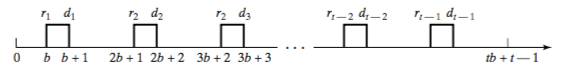
\includegraphics[width = 12cm]{Lmax1.png}

    図 $B.1$ : 各 $i \in \{1,\ldots,t - 1\}$ におけるジョブ $J_i$ のス
    ケジュール
  \end{center}
  各 $i \in \{1,\ldots,t - 1\}$ におけるジョブ $J_i$ を機械に割り当て
  たことで,区間 $[0,tb + t - 1]$ は長さ $b$ の $t$ 個の区間に分割され
  た.ここで,上記の条件を満たす $\mathcal{A} \subseteq 2^S$ が存在す
  ることから,$\forall A \in \mathcal{A}\big[|A| = 3 \land \sum_{a \in
  A}a = b \big]$ である.これより,各 $i' \in \{t,\ldots,4t - 1\}$ に
  おけるジョブ $J_{i'}$ は 長さ $b$ の $t$ 個の区間のいずれかに割り当
  てられる.また,各区間に割り当てられた 3 つのジョブの処理時間の和は
  $I_{(S,b)}$ より,$b$ である.

  以上より,上記の条件を満たす $\mathcal{A} \subseteq 2^S$ が存在するならば,
  $I_{(S,b)}$ を入力とする最大遅れ時間最小化問題に対して $\varphi(C) =
  0$ を満たす実行可能なスケジュール $C$ が存在する.
\end{proof}

\begin{lemma}\label{l_4}
  上記の条件を満たす $\mathcal{A} \subseteq 2^S$ が存在しないならば,$I_{(S,b)}$ を入力とする最大遅れ時間最小化問題に対して $\varphi(C) \le
  0$ を満たす実行可能なスケジュール $C$ が存在しない.
\end{lemma}

\begin{proof}
  各 $i \in \{1,\ldots,t - 1\}$ におけるジョブ $J_i$ は $r_i$ と $d_i =
  r_i + p_i$ の区間で処理される.(図 $B.1$)
  各 $i \in \{1,\ldots,t - 1\}$ におけるジョブ $J_i$ を機械に割り当て
  たことで,区間 $[0,tb + t - 1]$ は長さ $b$ の $t$ 個の区間に分割され
  た.ここで,上記の条件を満たす $\mathcal{A} \subseteq 2^S$ が存在し
  ないことから,$\forall A \in \mathcal{A}\big[|A| = 3 \land \sum_{a \in
  A}a \neq b \big]$ である.これより,各 $i' \in \{t,\ldots,4t - 1\}$ に
  おけるジョブ $J_{i'}$ は 長さ $b$ の $t$ 個の区間のいずれかに割り当
  てるとき,各区間のジョブの処理時間の和は $b$ ではない.
  以上より,上記の条件を満たす $\mathcal{A} \subseteq 2^S$ が存在しな
  いならば,$I_{(S,b)}$ を入力とする最大遅れ時間最小化問題に対して
  $\varphi(C) = 0$ を満たす実行可能なスケジュール $C$ は存在しない.
\end{proof}

補題~\ref{l_3} と補題~\ref{l_4} より,上記の条件を満たす$\mathcal{A} \subseteq 2^S$ が存在
することと,$I_{(S,b)}$ を入力とする最大遅れ時間最小化問題に対して
$\varphi(C) \le  0$
を満たす実行可能なスケジュール $C$ が存在することは,同値で
ある.
3 -PARTITION 問題の入力 $(S,b)$ に基づく $I_{(S,b)}$ の生成に要する計算時
間は,明らかに多項式時間であり,入力 $I_{(S,b)}$ の長さは,$(S, b)$
の長さに関する多項式で表すことができる.したがって,単一
機械モデルにおいて,最大遅れ時間最小化問題は強 NP 困難である.

\subsection{解法のまとめ}
処理開始可能時刻付き最大遅れ時間最小化問題は,各制約を緩めることで多項
式で最適解が求まることが証明されている.つまり,処理開始可能時刻付き最大遅れ時間最小化問題の部分問題に対して,多項式アルゴリズムが存在する.処理開始可能時刻と処理時間,納期の制約を緩和(ここでは,定数に設定)することで,多項式で最適解が求まる.
部分問題に対する解法は以下である.

\noindent\textbf{処理開始可能時刻の制約を緩めた場合( $\forall j \in \{1,\ldots,n\}\big[ r_j = r \big]$ )}

ジョブを納期の昇順で処理する( EDD ルール ) .つまり,スケジュールにおける任意の 2 つのジョブは以下の条件を満たす.
$$\forall i, j \in \{1,\ldots,n\}\big[d_i \le d_j \Rightarrow C(i) \le C(j)\big]$$


\noindent\textbf{処理時間の制約を緩めた場合( $\forall j \in \{1,\ldots,n\}\big[ p_j = p \big]$ )}

スケジュール可能なジョブの中で,納期が最も小さいジョブ順に処理する.つまり,スケジュールにおける各ジョブを順に $J_1,\ldots,J_n$,$C(0) = 0$ とすると,各ジョブは以下の条件を満たす.
$$\forall j, j' \in \bigg\{i \mid \forall i \in \{1,\ldots,n\}\big[r_i \le C(i - 1)\big]\bigg\}\bigg[j \le j' \Rightarrow d_j \le d_j'\bigg]$$

\noindent\textbf{納期の制約を緩めた場合( $\forall j \in \{1,\ldots,n\}\big[ d_j = d \big]$ )}

ジョブを処理開始可能時刻の昇順で処理する.つまり,スケジュールにおける任意の 2 つのジョブは以下の条件を満たす.
$$\forall i, j \in \{1,\ldots,n\}\big[r_i \le r_j \Rightarrow C(i) \le C(j)\big]$$

ここで,処理開始可能時刻を一定とした最大遅れ時間最小化問題の部分問題に対して,EDD ルールを適用することで最適解が求まることの証明を示す.


\begin{proof}
  スケジュール $S$ をある 2 つの連続するジョブについて納期順に並んでいな
  いジョブが存在するスケジュールとし,$S'$ をスケジュール $S$ において,
  2 つの連続するジョブについて納期順に並んでいな
  いジョブの位置を入れ替えたスケジュールとする.
  ただし,全てのジョブの処理時間は 0 以上とする.
  上記の条件をまとめた図は以下の通りである.
  \begin{center}
    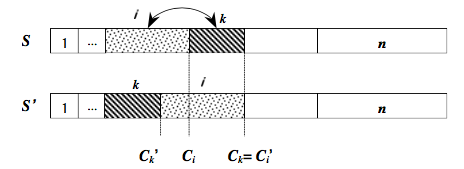
\includegraphics[width = 12cm]{EDDrule.png}
  \end{center}
  前提より,$d_i \ge d_k$ である.また,すべてのジョブの処理開始可能時
  刻が等しいことから,スケジュール $S$ における,ジョブ $J_i$ の処理開
  始時刻とスケジュール $S'$ におけるジョブ $J_k$ の処理開始時刻は等し
  い.つまり,$C_i - p_i = C'_k - p_k$ である.同様に,スケジュール
  $S$ における,ジョブ $J_k$ の完了時刻とスケジュール $S'$ におけるジョ
  ブ $J_i$ の完了時刻は等しい.つまり,$C_k = C'_i$ である.
  以上より,
  スケジュール $S$ のとき,$L_i(S) = C_i - d_i$,$L_k(S) = C_k - d_k$ ,
  スケジュール $S'$ のとき,$L_i(S') = C'_i - d_i = C_k - d_i \le C_k -
  d_k = L_k(S)$,$L_k(S') = C'_k - d_k \le C_k - d_k = L_k(S)$ と表すこ
  とができる.
  ここで,ジョブ $J_i,\ J_k$ を除いたジョブにおける最大遅れ時間を $L(S)$
  とする.つまり,$L(S) = \displaystyle \max_{j \in \{1,\ldots,n\}
  \setminus \{i,k\}}L_j(S)$.よって,スケジュール $S$,スケジュール
  $S'$ における最大遅れ時間はそれぞれ,次のように表すことができる.
  $$\left\{ \begin{array}{lll} L_{\max}(S) =
  \max\{L(S),L_i(S),L_k(S)\} \\ L_{\max}(S') =
  \max\{L(S),L_i(S'),L_k(S')\}\end{array} \right.$$
  今までの議論より,$L_{\max}(S') \le L_{\max}(S)$ であることは明らかで
  ある.また,スケジュールの全体集合を $\Pi$,EDD ルールを適用したスケ
  ジュールの集合を $\Pi^a$ とすると,
  前述の議論より,$\forall \pi \in \Pi$, $\exists \pi' \in \Pi^a$, $L_{\max}(\pi') \le
  L_{\max}(\pi)$ と表すことができる.また,どのスケジュールに対しても,
  EDD ルールを適用することで,一つの解に収束するので,
  $\forall \pi, \pi \in \Pi^a$, $L_{\max}(\pi) = L_{\max}(\pi')$ と表す
  ことできる.
  以上より,$\forall \pi \in \Pi$, $\forall
  \pi' \in \Pi^a$, $L_{\max}(\pi') \le L_{\max}(\pi)$ となる.
  つまり,全てのスケジュールは EDD ルールを適用することで,一つのスケジュー
  ルに収束し,そのスケジュールにおける解は他のどのスケジュールの解よりも
  悪くはならない.
  よって,EDD ルール $1\mid \mid L_{\max}$ 問題に対して,最適解を求める
  正しい解法である.
\end{proof}

全てのジョブにおける処理時間や納期が常に一定であるときも,同様に証明で
きる.この解法は,本研究で扱う最大実行開始待ち時間最小化問題の部分問題の解法に適用でき最適解を求めることができる.
第~\ref{c_5}~章では,部分問題の解法を利用した分枝限定法の紹介を行う.

\chapter{最大実行開始待ち時間最小化問題の計算複雑さ}\label{c_4}
最大実行開始待ち時間最小化問題は,どの機械モデルにおいても,計算複雑さ
が明らかでない.本研究では,無関連並列機械モデルにおける最大実行開始待
ち時間最小化問題(決定問題)が NP 完全であることを示した.
\section{NP完全性の証明}
3-SAT からの還元によって,この問題が NP  完全であることを示す.3-SAT
の定義は以下である.

\begin{description}
  \item[Instance : ] ブール型の変数集合 $X$ と,$X$ 上の 3 つのリテラル
  からなる集合の集合 $H$ (各 $h \in H$ は $|h| = 3$ を満たす).
  \item[Question : ] $H$ を充足する真理値割り当て $f ; X \to \{0,1\}$,
  つまり,
  $$\displaystyle \bigwedge_{h \in H} \bigg(\bigvee_{x \in h}f(x) \lor
  \bigvee_{\bar x \in h}\lnot f(x) \bigg) = 1$$
  を満たす $f$ が存在するか?
\end{description}

ブール型変数の集合 $X =\{x_1, x_2,\ldots ,x_n\}$ と, $X$ 上の 3 つのリテラルからなる集合の集合 $H =\{h_1, h_2,\ldots ,h_{\lambda}\}$ の 2 項組,$(X,H)$ を任意の 3-SAT 問題の入力とする.

各 $i \in \{1,2,\ldots, n\}$ について,$\alpha_i$ を $H$ に おいて $x_i$ が現れる回数を表す自然数とし,$\beta_i$ を $H$ において $\bar x_i$ が現れる回数を表す自然数とする.
つまり,$\alpha_i = \big|\{h \in H \mid x_i \in h\}\big|$,$\beta_i = \big|\{h \in H \mid \bar x_i \in h\}\big|$
また,$\displaystyle \sum_{i \in \{1,\ldots,n\}} \alpha_i = \mathcal{A}$, $\displaystyle \sum_{i \in \{1,\ldots,n\}} \beta_i = \mathcal{B}$  とする.

ただし,各 $i \in \{1,2,\ldots, n\}$ について,$\alpha_i$, $\beta_i$ は 3 以上とする.\\
つまり,$\forall i \in \{1,\ldots,n\}\big[\alpha_i \ge 3\big]$,
$\forall i \in \{1,\ldots,n\}\big[\beta_i \ge 3\big]$

$(X.H)$ に基づき,以下のように 最大実行開始待ち時間最小化問題の入力を設定する.
$2(\mathcal{A} + \mathcal{B}) + \lambda$ 個のジョブ $\mathcal{J}$ を
$n + \lambda$ 台の無関連機械で処理する.
\begin{itemize}
  \item $\mathcal{J}^t \subset \mathcal{J}$ s.t. $|\mathcal{J}^t| =
  \mathcal{A}  + \mathcal{B}$,
  \item $\mathcal{J}^f \subset \mathcal{J}$
  s.t.$|\mathcal{J}^f| = \mathcal{A}  + \mathcal{B}$,
  \item $\mathcal{J}^d \subset \mathcal{J}$ s.t.$|\mathcal{J}^d| =
  \lambda$
\end{itemize}
ただし,$\mathcal{J} = \mathcal{J}^t \cup \mathcal{J}^f \cup
\mathcal{J}^d$ ,$\mathcal{J}^t \cap \mathcal{J}^f = \emptyset$,$\mathcal{J}^f \cap \mathcal{J}^d = \emptyset$,$\mathcal{J}^d \cap \mathcal{J}^t = \emptyset$

つまり,$\{\mathcal{J}^t, \mathcal{J}^f,\mathcal{J}^d\}$ は $\mathcal{J}$ の分割である.

\begin{description}
  \item[実行開始待ち時間の設定:] $$w = 2$$
  \item[] まず,ジョブ $\mathcal{J}^d = \{J^d_1,\ldots,J^d_{\lambda}\}$ について,
  処理開始可能時刻関数 $r$ を以下のように設定する.
  $$r(\mathcal{J}^d) = 3(\mathcal{A} + \mathcal{B})$$
  処理時間関数 $p$ を以下のように設定する.
  $$p(\mathcal{J}^d, A(\mathcal{J}^d)) = 3$$

  次に,$2(\mathcal{A} + \mathcal{B})$ 個のジョブ $\mathcal{J}^t =
  \{J^t_1,\ldots,J^t_{\mathcal{A} + \mathcal{B}}\}$ と $\mathcal{J}^f =
  \{J^f_1,\ldots,J^f_{\mathcal{A} + \mathcal{B}}\}$ の処理開始可能時刻関
  数,処理時間関数を以下のように設定する.
  \item[処理開始可能時刻関数の設定:] 各機械 $i \in \{1,2,\ldots,n\}$ に対応させた各ジョブの処理時間関数を設
  定する.各ジョブを添え字の昇順に基づき $2n$ 個のグループに分ける. 各 $i
  \in \{1,2,\ldots,n\}$ における $i$ 番目のジョブの集合を
  $\mathcal{J}^t(i)$ とし,$n + i$ 番目のジョブの集合を
  $\mathcal{J}^f(i)$ とする.また,グループ $i$ の $\ell$ 番目のジョブ
  を $J^t(i,\ell)$ または $J^t(i,\ell)$ と表記する.
  \begin{itemize}
    \item ジョブの集合 $\mathcal{J}^t$ について, 各グループ $i \in
    \{1,2,\ldots, n\}$ の $\ell$ 番目のジョブの処理開始可能時刻関数を各
    $i$ における$\ell \in \{1,2,\ldots, \alpha_i + \beta_i\}$ について,
    以下のように設定する.
    $$r(J^t(i,\ell)) =
    \left\{ \begin{array}{lll} 3 \displaystyle
    \sum_{j \in \{1,\ldots,i - 1\}}(\alpha_j + \beta_j) + \ell - 1 &
    \text{if } \ell < \beta_i + 1, \\ 3 \displaystyle \sum_{j \in \{1,\ldots,i - 1\}}(\alpha_j + \beta_j) + \alpha_i + \ell - 2 & \text{otherwise} \end{array} \right.$$

    \item ジョブの集合 $\mathcal{J}^f$ について,各グループ $i \in \{1,2,\ldots, n\}$ の $\ell$ 番目のジョブの処理開始可能時刻を各 $i$ における $\ell \in \{1,2,\ldots,\alpha_i + \beta_i\}$ について,以下のように設定する.
    $$r(J^f(i,\ell)) =
    \left\{ \begin{array}{lll} 3 \displaystyle \sum_{j \in \{1,\ldots,i
    - 1\}}(\alpha_j + \beta_j) + \ell - 1 & \text{if } \ell = 1,
    \\ 3\displaystyle \sum_{j \in \{1,\ldots,i - 1\}}(\alpha_j + \beta_j) + \alpha_i + \ell  &
    \text{else if } \ell < \alpha_i + 1 , \\ 3\displaystyle \sum_{j \in \{1,\ldots,i - 1\}}(\alpha_j + \beta_j) + (\alpha_i + \beta_i + 4) + \ell & \text{otherwise} \end{array} \right.$$
  \end{itemize}
  \item[処理時間関数の設定:] 各ジョブを処理開始可能時刻の昇順に基づき $2n$ 個のグループに分ける
  \begin{itemize}
    \item グループ $i \in \{1,2,\ldots,n\}$ に機械 $i$ に対応させ,グループ
    $n + i$ にも同様に機械 $i$ を対応させる.各 $i \in \{1,2,\ldots,
    n\}$,$\ell \in \{1,2,\ldots, \alpha_i + \beta_i\}$ について,以下の
    ように設定する.ただし,機械 $i$ に対応しないジョブ,つまり,$A(\mathcal{J}^t)  \neq i$ のとき,ジョブ $J^t \in \mathcal{J}^t$ の処理時間は $3(\mathcal{A} + \mathcal{B}) + 3$ とする.
  \end{itemize}
  {\footnotesize
  $$p(J^t(i,\ell), A(\mathcal{J}^t)) =
  \left\{ \begin{array}{lllll} 1 & \text{if } \ell < \beta_i, \\
  \alpha_i + 4 & \text{if } \ell = \beta_i,\\ 1 & \text{if } \ell < \alpha_i + \beta_i, \\
  3(\mathcal{A} + \mathcal{B}) - \big\{ 3\displaystyle \sum_{j \in
  \{1,\ldots,i - 1\}}(\alpha_j + \beta_j) + (2\alpha_i +
  \beta_i - 2)\big \} + 3 & \text{if } \ell = \alpha_i +
  \beta_i \end{array} \right.$$
  }
  {\footnotesize
  $$p(J^f(i,\ell),A(\mathcal{J}^f)) = \left\{ \begin{array}{lllll}
  \beta_i + 2 & \text{if } \ell = 1, \\
  1 & \text{if } \ell < \alpha_i, \\ \alpha_i
  + 5 & \text{if } \ell = \alpha_i , \\ 1 & \text{if } \ell < \alpha_i + \beta_i, \\ 3(\mathcal{A} + \mathcal{B}) -
  \big\{ 3\displaystyle \sum_{j \in \{1,\ldots,i - 1\}}(\alpha_j + \beta_j)
  + (2\alpha_i + 2\beta_i + 4)\big \} + 3 & \text{if }
  \ell = \alpha_i + \beta_i \end{array} \right.$$
  }
  \begin{itemize}
    \item 残りの各機械 $k \in \{n + 1, \ldots , n + \lambda\}$ について,
    各ジョブの処理時間を設定する
    各グループ $i \in \{1,2,\ldots,n\}$ について $x_i$ を対応させ,グ
    ループ $n + i$ について $\bar x_i$ を対応させる.つまり,$\forall
    i \in \{1,\ldots,n\}\big[x_i \to \mathcal{J}^t(i),\ \bar x_i \to
    \mathcal{J}^f(i) \big]$,
    $\mathcal{J}^t(i) = \big\{J^t(i,1),\ldots,J^t(i,\alpha_i +
    \beta_i)\big\}$,$\mathcal{J}^f(i) =
    \big\{J^f(i,1),\ldots,J^f(i,\alpha_i + \beta_i)\big\}$.
    各 $k \in \{n + 1, \ldots , n + \lambda\}$ について,
    $h_{k - n}$ に含まれるリテラルに対応するジョブを処理開始可能時刻の
    昇順で $\mathcal{T}(h_{k - n})$, $\mathcal{F}(h_{k - n})$ に入れる.
    $x_i \in h_{k - n}$ のとき,グループ $\mathcal{J}^t(i)$ のジョブを
    $\beta_i + 1$ 番目から順に $\mathcal{T}(k - n)$ に,
    $\mathcal{J}^f(i)$ のジョブを 1 番目から順に $\mathcal{F}(k - n)$ に加える.
    また,$\bar x_i \in h_{k - n}$ のとき,グループ $\mathcal{J}^f(i)$
    のジョブを $\alpha_i + 1$ 番目から順に $\mathcal{T}(k - n)$ に,
    $\mathcal{J}^t(i)$ のジョブを 1 番目から順に $\mathcal{F}(k - n)$ に加える.
    つまり,各 $k \in \{n + 1, \ldots,n + \lambda\}$,各 $i \in \{1,\ldots,n\}$
    について,$count(x_i,h_j) = \big|\big\{x_i \in h_l \mid l \in \{1,\ldots,j -
    1\}\big\}\big|$ を用いて,
  \end{itemize}
  \begin{equation}
    \begin{split}
      \mathcal{T}(h_{k - n}) &= \bigg\{\big\{J^t(i,\beta_i + 1 +
      count(x_i,h_{k - n})) \mid x_i \in h_{k - n}\big\} \cup \\ &\qquad \qquad\qquad \big\{J^f(i,\alpha_i + 1 + count(\bar x_i, h_{k - n})) \mid \bar x_i \in h_{k - n}\big\}\bigg\} \notag
    \end{split}
  \end{equation}
  \begin{equation}
    \begin{split}
      \mathcal{F}(h_{k - n}) &= \bigg\{\big\{J^f(i,1 + count(
      x_i,h_{k - n})) \mid x_i \in h_{k - n} \big\} \cup \\ &\qquad\qquad\qquad \big\{J^t(i,1 + count(\bar x_i,h_{k - n})) \mid \bar x_i \in h_{k - n}\big\} \bigg\} \cup J^d_{k - n} \notag
    \end{split}
  \end{equation}

  このとき,$i \in \{1,2,\ldots,n\}$,$k \in \{n + 1, \ldots , n +
  \lambda\}$,$\ell \in \{1,2,\ldots, \alpha_i + \beta_i\}$ について,
  処理時間関数を次のように設定する.
\end{description}
{\small
$$p(J,A(J)) = \left\{ \begin{array}{lll} \min \big\{r(J') \mid
J' \in \mathcal{F}(h_{k - n}) \wedge \big(r(J') > r(J) \big) \big\} - r(J)
& \text{if } J \in \mathcal{T}(h_{k - n}), \\ \min \big\{r(J') \mid
J' \in \mathcal{F}(h_{k - n}) \wedge \big(r(J') > r(J) \big) \big\} - r(J)
+ (4 - |h_j|) & \text{if } J \in \mathcal{F}(h_{k - n}), \\ 3(\mathcal{A} + \mathcal{B}) + 3 & \text{otherwise}\end{array} \right.$$
}

このように設定した $(p,r,w)$ は最大実行開始待ち時間最小化問題の入力である.以降,$(X,H)$ に基いて前述のように設定した $(p,r,w)$ を区別して $I_{(X,H)}$ と表す.( $I_{(X,H)} = (p,r,w)$ )

以下, $H$ を充足する真理値割り当て $f : X \to \{0,1\}$ が存在する
ことと,$I_{(X,H)}$ を入力とする最大実行開始待ち時間最小化問題に対し
て,$\varphi(A,s) \le 2$ を満たす実行可能なスケジュール $(A,s)$ が
存在することが,同値であることを示す.

\begin{lemma}\label{l_5}
  $H$ を充足する真理値割り当て $f : X \to \{0,1\}$ が存在するならば,$I_{(X,H)}$ を入力とする最大実行開始待ち時間最小化問題に対して
  $\varphi(A, S) \le 2$ を満たす実行可能なス
  ケジュール $(A, S)$ が存在する.
\end{lemma}

\begin{proof}
  各 $i \in \{1,\ldots, n\}$ について,$f(x_i) = 1$ ならばグループ $n +
  i$ の全てのジョブを,グループ $n + i$ に対応する機械 $i$ に割り当て,
  そうでなければグループ $i$ の全てのジョブを,グループ $i$ に対応する機
  械 $i$ に割り当てる.つまり,各 $i \in \{1,\ldots, n\}$ における各
  $\ell \in \{1,\ldots,\alpha_i + \beta_i\}$ について,
  $f(x_i) = 1$ ならば,$A_i := A_i \cup \mathcal{J}^f(i)$
  $f(x_i) = 0$ ならば,$A_k := A_k \cup \mathcal{J}^t(i)$
  $I_{(X,H)}$ の定義より,ここまでのスケジュールにおいて,機械
  $\{1,\ldots, n\}$ に割り当てたジョブは処理開始可能時刻と納期の間で重複せず処理される.
  よって,このとき,機械 $\{1,2,\ldots,n\}$ に割り当てられた
  $\mathcal{A} + \mathcal{B}$ 個のジョブの実行開始遅れ時間は $0$ である.

  上述の割り当てにより,各 $i \in \{1,\ldots,n\}$ について,$x_i$ または
  $\bar x_i$ に対応するジョブ $\mathcal{J}^t(i)$ または
  $\mathcal{J}^f(i)$ のどちらか一方が機械 $i$ に割り当てられた.このとき,
  上図より,機械 $i$ におけるジョブの完了時刻は $3(\mathcal{A} +
  \mathcal{B}) + 3$ であるので,いずれのジョブも機械 $i$ に割り当てることができない.
  よって,残りのジョブについては,各 $k \in \{n + 1,\ldots,n +
  \lambda\}$ における機械 $k$ に割り当てる.

  前提条件より,$f$ が $H$ を充足することから,各 $i \in \{1,\ldots,n\}$,
  $j \in \{1, \ldots, \lambda \}$ について,$f(x_i) = 1$ を満たす $x_i
  \in h_j$ か,$f(x_i) = 0$ を満たす $\bar x_i \in h_j$ を満たすリテラルは必ず存在する.
  ここで,与えられた $j \in \{1, \ldots, \lambda \}$ について,$f(x_i) =
  1$ を満たす $x_i \in h_j$ を見つけたと仮定する.グループ $i$ のジョブ
  の集合 $\mathcal{J}^t(i)$ は,$f(x_i) = 1$ であることから,
  $\{1,\ldots,n\}$ のいずれの機械にも割り当てられていないので,そのよう
  なグループ $i$ のジョブの集合 $\mathcal{J}^t(i)$ は必ず存在する.
  同様に,$f(x_i) = 0$ を満たす $\bar x_i \in h_j$ を見つけたと仮定する.
  グループ $n + i$ のジョブの集合 $\mathcal{J}^f(i)$ のうち,いずれの機
  械にも割り当てられていないグループ $n + i$ を見つける.先程と同じ議論
  で,そのようなグループ $n + i$ のジョブ $\mathcal{J}^f(i)$ は必ず存在する.

  各 $j \in \{1, \ldots, \lambda \}$ における $h_j$ に対応するジョブの集
  合 $\mathcal{T}(h_j)$ または $\mathcal{F}(h_j)$ のジョブを処理開始可能
  時刻の昇順で機械 $j$ に割り当てる.
  このとき,1 に割り当てられたリテラルに対応するジョブが少なくとも 1 つ
  各機械に割り当てられているので,各機械におけるジョブの完了時刻は高々
  $3(\mathcal{A} + \mathcal{B}) + 2$ である.
  ここで,各 $j \in \{1,\ldots,\lambda\}$ における $J^d_j$ を各機械 $j$
  に 1 つずつ割り当てる.
  このとき,$J^d$ の処理開始可能時刻は $I_{(X,H)}$ より,$3(\mathcal{A}
  + \mathcal{B})$ であるので,実行開始待ち時間は高々 2 である.

  今までの議論より,$\mathcal{A} + \mathcal{B}$ 個のジョブを機械 $i \in
  \{1,\ldots,n\}$ に,$\mathcal{A} + \mathcal{B}$ 個のジョブを機械 $k \in\{n + 1, \ldots, n + \lambda\}$ に,$\lambda$ 個のジョブを機械 $k \in\{n + 1, \ldots, n + \lambda\}$ に割り当てた.
  このとき,全てのジョブをいずれかの機械に割り当てており,全てのジョブに
  関して,実行開始待ち時間は高々 2 であることから,$f$ が $H$ を充足す
  るとき,$I_{(X,H)}$ において,$\varphi(A,s) \le 2$ を満たす.
\end{proof}

\begin{lemma}\label{l_6}
  $H$ を充足する真理値割り当て $f : X \to \{0,1\}$ が存在しないならば,$I_{(X,H)}$ を入力とする最大実行開始待ち時間最小化問題に対して
  $\varphi(A, C) \le 2$ を満たす実行可能なス
  ケジュール $(A, S)$ が存在しない.
\end{lemma}

\begin{proof}
  $f$ が $H$ を充足しないことから,各 $j \in \{1, \ldots, \lambda \}$ に
  ついて,$f(x_i) = 1$ を満たす $x_i \in h_j$ か,$f(x_i) = 0$ を満たす
  $\bar x_i \in h_j$ が1つも存在しない機械 $j \in \{1,\ldots, \lambda\}$ が必ず存在する.
  その機械を $j^{\prime}$ とし,以下,機械 $j^{\prime}$ 上のスケジュールについて述べる.
  \begin{itemize}
    \item $x_i \in h_j^{\prime}$ または $\bar x_i \in h_j^{\prime}$ に対応
    するジョブのみを機械 $j^{\prime}$ に割り当てた場合
    \begin{itemize}
      \item $|h_j^{\prime}| = 3$ のとき,

      $I_{(X,H)}$ より,それらのジョブは,スケジュールにおける次のジョブ
      の処理開始可能時刻を 1 超える処理時間を持つ.$h_{j^{\prime}}$ に含
      まれる $x_i$ 以外の残りの 2 つのリテラルに対応するジョブについても
      同様に機械 $j^{\prime}$ に割り当てる.
      $I_{(X,H)}$ より,機械 $j^{\prime}$ におけるジョブの完了時刻は
      $3(\mathcal{A} + \mathcal{B}) + 3$ となる.ここで,$j \in
      \{1,\ldots,\lambda\}$ におけるジョブ $J^d_{j^{\prime}}$ をそれらの
      ジョブの後に割り当てるとき,ジョブ $J^d_{j^{\prime}}$ に 3 の実行開始待ち時間が発生する.
      \item $|h_j^{\prime}| = 2$ のとき,

      $|h_j^{\prime}| = 3$ のときと同様に割り当てる.$I_{(X,H)}$ より,
      各ジョブはスケジュールにおける次のジョブの処理開始可能時刻を 2 超
      える処理時間を持つ.$h_{j^{\prime}}$ に含まれる $x_i$ 以外の残りの
      1 つのリテラルに対応するジョブについても同様に機械 $j^{\prime}$ に割り当てる.
      $I_{(X,H)}$ より,機械 $j^{\prime}$ におけるジョブの完了時刻は
      $3(\mathcal{A} + \mathcal{B}) + 4$ となる.ここで,$j \in
      \{1,\ldots,\lambda\}$ において,機械に割り当てられていないジョブ
      $J^d_{j^{\prime}}$ をそれらのジョブの後に割り当てるとき,ジョブ
      $J^d_{j^{\prime}}$ に 4 の実行開始待ち時間が発生する.
      \item  $|h_j^{\prime}| = 1$ のとき,

      $|h_j^{\prime}| = 3$ のときと同様に割り当てる.$I_{(X,H)}$ より,
      各ジョブはスケジュールにおける次のジョブの処理開始可能時刻を 3 超える処理時間を持つ.
      $I_{(X,H)}$ より,機械 $j^{\prime}$ におけるジョブの完了時刻は
      $3(\mathcal{A} + \mathcal{B}) + 3$ となる.ここで,$j \in
      \{1,\ldots,\lambda\}$ において,機械に割り当てられていないジョブ
      $J^d_{j^{\prime}}$ をそれらのジョブの後に割り当てるとき,ジョブ
      $J^d_{j^{\prime}}$ に 3 の実行開始待ち時間が発生する.
    \end{itemize}
    \item $x_k \notin h_j$ または $\bar x_k \notin h_j$ に対応するジョブを
    割り当てた場合

    機械 $j^{\prime}$ にそのようなジョブを1 つでも割り当てた場合,
    $I_{(X,H)}$ より,機械 $j^{\prime}$ におけるジョブの完了時刻は
    $3(\mathcal{A} + \mathcal{B}) + 3$ となる.ここで,$j \in
    \{1,\ldots,\lambda\}$ において,機械に割り当てられていないジョブ
    $J^d_{j^{\prime}}$ をそれらのジョブの後に割り当てるとき,ジョブ
    $J^d_{j^{\prime}}$ に 3 の実行開始待ち時間が発生する.
    \item 上記の 2 つのケースにおいて,$j \in \{1,\ldots,\lambda\}$ におい
    て,機械に割り当てられていないジョブ $J^d_{j^{\prime}}$ を機械 $i
    \in \{1,\ldots,n\}$ に割り当てた場合 $I_{(X,H)}$ より,ジョブ
    $J^d_{j^{\prime}}$ に 3 の実行開始待ち時間が発生する.
  \end{itemize}
  以上より,各 $j \in \{1,\ldots,\lambda\}$ における機械 $j$ にどのジョ
  ブをどのように割り当てたしたとしても,少なくとも 1 つ実行開始待ち時間が3以上になる機械が存在する.
  よって,$H$ を充足する真理値割り当て $f$ が存在しないとき,実行開始待
  ち時間が 2 以下となるスケジュールは存在しない.
\end{proof}

補題~\ref{l_5} と補題~\ref{l_6} より,$H$ を充足する真理値割り当て $f : X \to \{0,
1\}$ が存在することと,$I_{(X,H)}$ を入力とする最大実行開始待ち時間
最小化問題に対して $\varphi(A, S) \le 2$
を満たす実行可能なスケジュール $(A, S)$ が存在することは,同値で
ある.
3 -SAT 問題の入力 $(X,H)$ に基づく $I_{(X,H)}$ の生成に要する計算時
間は,明らかに多項式時間であり,入力 $I_{(X,H)}$ の長さは,$(X, H)$
の長さに関する多項式で表すことができる.したがって,無関連並列
機械モデルにおいて機械数が入力の一部の場合, 最大実行開始待ち時間
最小化問題は NP 完全である.

\section{機械モデルの違いが計算複雑さに与える影響}
最大実行開始待ち時間最小化問題(決定問題)に対して,以下のことが明らかになった.
\begin{itemize}
  \item 単一機械モデル
  \begin{itemize}
    \item $w = 0$ のとき,多項式で判定可能.
    \item $w \neq 0$ のとき,明らかでない.
  \end{itemize}
  \item 同一並列機械モデル
  \begin{itemize}
    \item $w = 0$ のとき,多項式で判定可能.
    \item $w \neq 0$ のとき,明らかでない.
  \end{itemize}
  \item 一様並列機械モデル
  \begin{itemize}
    \item 明らかでない.
  \end{itemize}
  \item 無関連並列機械モデル
  \begin{itemize}
    \item 機械数が入力の一部の場合,NP 完全.
    \item 機械数が定数の場合,明らかでない.
  \end{itemize}
\end{itemize}

単一機械モデルにおける最大実行開始待ち時間最小化問題(決定問題)について,$w = 0$ のとき,多項式で判定可能であることを示す.

以下の条件を満たすとき,決定問題の解は Yes,満たさないとき No であることは明らかである.
$$\forall J,J' \in \mathcal{J}\big[[r(J),r(J) + p(J)) \cap [r(J'),r(J') + p(J')) = \emptyset\big]$$
$w = 0$ となるスケジュールとは,すべてのジョブが処理開始可能時刻と 処理開始可能時刻 + 処理時間 の間で処理されなければならない.つまり,すべてのジョブに関して各ジョブの [処理開始可能時刻,処理開始可能時刻 + 処理時間] で表される範囲が被ってはいけない.この判定にかかる時間は高々 $\mathcal{O}(n^2)$ であることから,多項式時間で判定が可能である.


同様に,同一並列機械モデルにおける最大実行開始待ち時間最小化問題(決定問題)についても多項式で判定可能である.

%以下の条件を満たすとき,決定問題の解は Yes,満たさないとき No であることは明らかである.
%$$\bigg|\bigg\{ J \cup J' \mid \forall J,J' \in \mathcal{J}\big[[s(J),s(J) + p(J)) \cap [s(J'),s(J') + p(J')) \neq \emptyset\big]\bigg\}\bigg| \le |\mathcal{M}|$$

第 \ref{c_2} 章で記述した通り,各ジョブを処理する機械の性能によって,機械モデルは次のように分類され
る.まず,ジョブを処理する機械の台数について,一つの機械で処理する単一
機械モデルと,複数の機械で処理を行なう並列機械モデルに分類される.並列
機械モデルはさらに,全ての機械の性能が等しい同一並列機械モデル,機械ご
とに処理速度が異なる一様並列機械モデル,ジョブと機械の組み合わせによっ
て処理時間が異なる無関連並列機械モデルに分類される.ここで,各機械モデル間の関係を示す.

同一並列機械について,各機械の性能が等しいことから,単一機械の集合として扱うことができる.よって,単一機械モデルは,同一並列機械モデルの一部として捉えることができる.

同様に,同一並列機械,一様並列機械,無関連並列機械モデルについて,同一並列機械モデルは,一様並列機械モデルの中で機械の性能が等しいとき,一様並列機械モデルは無関連並列機械モデルの中で機械によって性能が変わるとき,つまり,同一並列機械モデルは一様並列機械モデルの一部として,一様並列機械モデルは無関連並列機械モデルの一部として捉えることができる.

つまり,単一機械モデルにおける最大実行開始待ち時間最小化問題が NP 完全であれば,残りの機械モデルにおけるスケジューリング問題についても NP 完全であることが言える.
しかし,本研究では,無関連並列機械モデルにおける NP 完全性のみ明らかにしたため,他の機械モデルにおける問題の計算複雑さは明らかでない.

単一機械モデルにおける最大実行開始待ち時間最小化問題(決定問題)は第~\ref{c_3} 章で紹介した,処理開始可能時刻つき最大遅れ時間最小化問題と対応する.しかし,最大実行開始待ち時間最小化問題(決定問題)は,処理開始可能時刻と納期が関連づけられている.処理開始可能時刻付き最大遅れ時間最小化問題により制限を加えた問題であると言える.つまり,最大実行開始待ち時間最小化問題は最大遅れ時間最小化問題の部分問題として捉えることができる.第~\ref{c_3}~章より,最大遅れ時間最小化問題が強 NP 困難であることから,最大実行開始待ち時間最小化問題も NP 困難であることが考えられるが,証明はできていない.

次の章では,同一並列機械モデルにおける最大実行開始待ち時間最小化問題に対して,適用する解法の紹介を行う.
また,分枝限定法を計算効率を向上させるために改良した点についても紹介する.

\chapter{実験的評価}\label{c_5}
この章では,提案する解法の紹介と,その解法の評価をするために用いる分枝限定法について紹介する.また,提案解法を用いて求めた解と分枝限定法を用いて求めた最適解を比較し,提案解法の質の分析を行った.

\section{本研究の提案解法}
本研究では,同一並列機械モデルにおける最大実行開始待ち時間最小化問題に対して,貪欲アルゴリズムを用いた解法を提案する.

%オンライン環境の説明
本研究の背景として,計算サーバーへのタスク割り当てを例に挙げて紹介した.
計算サーバーへのタスク割り当ては最大実行開始待ち時間を最小化するオンラインスケジューリング問題として捉えることができる.
オンラインスケジューリング問題とは,オンライン環境でのスケジューリング問題のことである.
オンライン環境とは,タスク(ジョブ)の情報があらかじめわからない環境を
さす.つまり,現時点で,いくつのタスク(ジョブ)を処理する必要があるの
か,各タスク(ジョブ)の処理時間はどのくらいなのかがわからない.よって,
このような環境では,タスクをどの順番で処理するかではなく,タスクの処理
要求が計算サーバーに届いた順で処理を開始するという方法が取られることは自然である.タスクの処理要求が計算サーバーに届いた順とは,各タスクの処理開始可能時刻順で処理することである.本研究の提案解法はこの考え方をもとにしている.

%参考文献調べる
このような考え方は,貪欲的解法と呼ばれ,最適化問題に対する最も単純なアルゴリズムの 1 つとして知られている.
バックトラッキングや局所探索と類似点は,実行可能解($p_1\ldots,p_n$)($i \in \{1,\ldots,n\}[p_i \in P_i]$)の仕様が必要であり,任意の貪欲アルゴリズムは局所ステップの系列と見ることができる点である.しかし,貪欲アルゴリズムは 1 つの実行可能解からもう 1 つの実行可能解には遷移しない.まず,空の状態から始まり,仕様における 1 つの局所パラメータを永久に確定する.第 2 ステップでは,局所アルゴリズムは仕様における第 2 のパラメータを確定する.この操作が実行可能解の完全な仕様に到達するまで繰り返される.貪欲アルゴリズムは,次の局所仕様を生成するために全ての可能性の中から最も有望と思われるパラメータを選択する.後で,どのような状況が起ころうと,この決定は決して変えられることはない.
また,貪欲アルゴリズムはバックトラッキングで生成される木
$T_{\mathcal{M}(x)}$ における根から葉までのちょうど 1 つの路を実現して
いる.空仕様は全ての実行可能解の集合 $\mathcal{M}(x)$ を考えており,
$\mathcal{M}(x)$ が木 $T_{\mathcal{M}(x)}$ における根のラベルであるこ
とを意味している.第 1 のパラメータ $p_1$ を指定することは,
$\mathcal{M}$ を集合 $S(p_1) = \{\alpha \in \mathcal{M}(x) \mid \alpha
\text{の仕様の第 1 パラメータは} p_1\}$ に制限することに対応する.
この手続きを繰り返すと,実行可能解の集合の系列
$$\mathcal{M}(x) \supseteq S(p_1) \supseteq S(p_1,p_2) \supseteq
\ldots, \supseteq S(p_1,p_2,\ldots,p_n)$$
を得る.ここで,$|S(p_1,p_2,\ldots,p_n)| = 1$ である.

以下の {\sc greedy Algorithm} が本研究の提案解法である.
インスタンス $I = (\mathcal{J}, \mathcal{M}, r, p)$
\begin{itemize}
  \item ジョブの集合 $\mathcal{J} = \{J_1,\ldots,J_n\}$
  \item 機械の集合 $\mathcal{M} = \{M_1,\ldots,M_m\}$
  \item ジョブの処理開始可能時刻を返す関数 $r : \mathcal{J} \to \mathbb{N}$
  \item ジョブの処理時間を返す関数 $p : \mathcal{J} \to \mathbb{N}$
\end{itemize}

\begin{quote}
  \begin{description}
    \item[\sc Algorithm : ] {\sc greedy Algorithm}
    \item[入力 :] $I = (\mathcal{J}, \mathcal{M}, r, p)$
    \item[出力 :] スケジュールの集合 $\mathcal{S}$,$\mathcal{S}$ における最大実行開始待ち時間 $W$.ただし $|\mathcal{S}| = |\mathcal{M}| = m$
    \begin{description}
      \item[Step 1.]
      $\mathcal{J}$ を処理開始可能時刻の昇順でソートする.
      \item[Step 2.]
      ここで,以下の変数を定義する.
      \begin{itemize}
        \item 各機械 $M \in \mathcal{M}$ のスケジュール $S_M \in \mathcal{S}$ におけるジョブの集合 $\mathcal{J}_{S_M}$ の集合 $\mathcal{J}Set$.ただし,$$\forall M, M' \in \mathcal{M}\big[M \neq M' \Rightarrow \mathcal{J}_{S_M} \cap \mathcal{J}_{S_M'} = \emptyset \big]$$ を満たす.つまり,$\mathcal{J}_{S_M}$ は $\mathcal{J}Set$ の分割である.
        \item 各機械 $M \in \mathcal{M}$ のスケジュール $S_M \in \mathcal{S}$ における完了時刻 $C(\mathcal{J}_{S_M})$ の集合 $\mathcal{C}$.ここで,完了時刻を返す関数 $C : \mathcal{J} \to \mathbb{N}$ を定義する.
        \item 各機械 $M \in \mathcal{M}$ のスケジュール $S_M \in \mathcal{S}$ における最大実行開始待ち時間 $w(S_M)$ の集合 $\mathcal{W}$.ここで,最大実行開始待ち時間を返す関数 $w : S \to \mathbb{N}$ を定義する.
      \end{itemize}

      \item[Step 3.]
      各 $i \in \{1,\ldots,n\}$ における $J_i$ について,$i = 1$から順に以下の処理を繰り返す
      \begin{description}
        \item[Step 3.1.]
        $M_a = \big\{M \mid \forall M, M' \in \mathcal{M}, \min\{C(S_M), C(S_M')\}\big\}$ \\ただし,$|M_a| = 1$.
        つまり,$\mathcal{C}$ のなかで最小の完了時刻を持つ機械を
        $M_a$ とする.ここで,
        $\mathcal{J}_{S_{M_a}} := \mathcal{J}_{S_{M_a}} \cup J_i$,$S_{M_a} := S_{M_a} \cup J_i$ とする.
      \end{description}

      \item[Step 4.]
      ここで,$\mathcal{S} = \{ S_M \mid \forall M \in \mathcal{M}\}$,$W = w(\mathcal{S})$ として,$\mathcal{S},W$ を出力する.
    \end{description}
  \end{description}
\end{quote}

上記 {\sc greedy Algorithm} は,処理開始可能時刻が最も早いジョブから順に,処理をしていない機械に割り当てる.Step 2. で定義している $\mathcal{C}$ と $\mathcal{W}$ は機械ごとに,その時点での完了時刻と最大実行開始待ち時間を格納する.
Step 3. では,$\mathcal{C}$ の中で,最小の完了時刻を持つ機械を取得し,$M_a$ と定義する.
その後,ジョブの集合 $\mathcal{J}_{S_{M_a}}$ にジョブ $J_i$ を追加する.

\section{分枝限定法による評価}
分枝限定法は最適化問題に対するアルゴリズムを設計するための方法である.この方法は計算時間がどうであろうと,無条件で最適解を見つけたいときに用いる.分枝限定法は,すべての実行可能解の空間をしらみつぶしに探索する手法のバックトラッキングに基づいている.分枝限定法の大まかなアイデアは,しらみつぶし探索において,解を生成するある部分に達したとき,その部分に最適解が含まれていないことがわかったときには,実行可能解の空間のその部分の探索を省略することによってバックトラッキングを早くすることである.

ここで,バックトラッキングを適用するための表記法を導入する.
$\mathcal{M}(x)$ を最適化問題の入力インスタンス $x$ に対するすべての実行可能解の集合とする.$T_{\mathcal{M}(x)}$ を以下のような性質を持つラベル付き木と定義する.
\begin{itemize}
  \item $T_{\mathcal{M}(x)}$ の任意の頂点 $v$ は集合 $S_v \subseteq \mathcal{M}(x)$ によってラベル付けられている.
  \item $T_{\mathcal{M}(x)}$ の根は $\mathcal{M}(x)$ によってラベル付けられている.
  \item $T_{\mathcal{M}(x)}$ において $v_1,\ldots,v_m$ が $v$ の親の全ての子であるならば,$$\forall i,j \in \{1,\ldots,m\}\bigg[i \neq j \Rightarrow S_v = \bigcup_{i = 1}^{m}S_{v_i} \land S_{v_i} \cap S_{v_j} = \emptyset \bigg]$$ が成り立つ.つまり,$v$ は $S_v$ の分割である.
  \item $T_{\mathcal{M}(x)}$ の各葉 $u$ に対して,$|S_u| \le 1$.つまり,葉が$\mathcal{M}(x)$ の実行可能解に対応している.
\end{itemize}

バックトラッキングは,ラベルの付いた根付き木 $T_{\mathcal{M}(x)}$ に対する深さ優先探索,あるいは幅優先探索とみなすことができる,ここで葉は $\mathcal{M}(x)$ からの実行可能解でラベル付けされており,$T_{\mathcal{M}(x)}$ の全ての内部頂点 $v$ には,$v$ を根とする部分木 $T_v$ の葉のラベルが付いた全ての実行可能解を含む $S_v \subseteq \mathcal{M}(x)$ でラベル付けされている.分枝限定法は,アルゴリズムが $v$ を訪れた時点で,$T_v$ が最適解を持たないこと決定できるときに,$T_{\mathcal{M}(x)}$ から $T_v$ を切り取ることに他ならない.このアプローチの効率はアルゴリズムの実行中に切断され得る $T_{\mathcal{M}(x)}$ の部分木の量とサイズに依存する.

分枝限定法は多くの NP 困難な組合わせ最適化問題に対して,その最適解を求めるための最も良い
枠組みとして知られており,Land and Doig [1960] \cite{BandB} によって
提案され,Little, Murty, Sweeney and Karel [1963] \cite{BandB2}
によって TSP にはじめて適用されている.

分枝限定法の最も単純な版は,頂点 $v$ に到達したとき,それまでに見つかった最良のコストと $T_v$
の $S_v$ における実行可能解の最小または最大(ここでは最大)のコストを比較する.それまでの最良のコストが評価された範囲のどのコストよりも明らかに良ければ,$T_v$ を切り取る(すなわち, $T_v$ の探索を中断する).

%図入れたほうがいいかもしれない

この節では,同一並列機械モデルにおける最大実行開始待ち時間最小化問題に対する分枝限定法のアルゴリズムを紹介する.分枝限定法によるアプローチの効率はアルゴリズムの実行中に切断される $T_{\mathcal{M}(x)}$ の部分木の量とサイズ,プログラムに依存するため,本研究で作成した分枝限定法のアルゴリズムは,分割生成方法と探索を続行するか中断するかの判定部分を改良した.%また,順列の生成に用いるデータ構造を双方向リストとした.双方向リストの各ノードには 2 つのリンクがあり,1 つが次のノード(ここでは,$.next$ と表記する),もう 1 つが前のノード(ここでは,$.previous$ と表記する)を指す.またここでは,先頭のノードを $head$ と表記し,双方向リストの最後尾のノードの次のノードを $head$,$head$ の前のノードを双方向リストの最後尾のノードとする.

以下では,分割の生成方法,分枝限定法のアルゴリズムと工夫部分について,紹介する.その後,アルゴリズムの紹介を行う.
分割の生成方法については Kreher. Donald L.(1998) \cite{Partition} に
よって,紹介されている.

同一並列機械の場合,全ての機械の性能が同じであることから,ジョブをどの機械に割り当てたとしても,処理時間は変わらない.そのため,同一並列機械では,どの機械に割り当てるかではなく,どのジョブと同じ機械で処理するかを考える必要がある.
各ジョブの処理は任意の 1 機械で処理を完了するため,同一並列機械へのジョブの割り当ては,ジョブの分割として捉えることができる.分割の定義は以下である.$\mathcal{J}$ の分割 $\Pi$ の要素 $\pi \in \Pi$ に対して,以下の条件を満たす $\Pi$.
\begin{itemize}
  \item $\displaystyle \bigcup_{\pi \in \Pi}\pi = \mathcal{J} $
  \item $\forall \pi, \pi' \in \Pi \big[\pi \neq \pi' \Rightarrow \pi \cap \pi' = \emptyset \big]$
\end{itemize}

%実装部分での工夫と,アルゴリズム部分での工夫は分ける
議論に先立ち,表記を導入する.コストの下限を返す関数を $cost : \mathcal{J} \to \mathbb{N}$ とする.また,$M = \pi$ は分割の要素 $\pi$ に機械 $M$ が対応することを意味する.
\begin{description}
  \item[分割生成アルゴリズムの改良] ~
  \begin{itemize}
    \item $|\Pi| = |\mathcal{M}|$ を満たす分割 $\Pi$ のみ生成した.

    \item 各 $\pi \in \Pi$ における $\mathcal{J}_{\pi}$ のコストの下限 $cost(\mathcal{J}_{\pi})$ を評価し,分割 $\Pi$ において,スケジュールを生成するかどうかの判定を追加した.

    \item 各 $\pi \in \Pi$ における $cost(\mathcal{J}_{\pi})$ を降順でソートし,順に $\pi$ に対応する機械にジョブ $J \in \mathcal{J}_{\pi}$ を割り当てる.

  \end{itemize}
  \item[分枝限定法アルゴリズムの改良] ~
  \begin{itemize}
    \item $cost(\mathcal{J}_{M_a} \setminus \mathcal{J}_{S_{M_a}})$を評価し,探索を続行するか中断するかの判定を追加した.機械 $M_a = \pi \in \Pi$ において,$M_a$ に割り当てられたジョブの集合を $\mathcal{J}_{S_{M_a}}$ とする.
  \end{itemize}
\end{description}

以下では,上記改良を加えた分割生成アルゴリズムと,分枝限定法アルゴリズムの紹介を行う.
議論に先立ち表記の導入を行う.ジョブの集合を $\mathcal{J}$,ジョブ数を $n(=|\mathcal{J}|)$,機械数を $m(=|\mathcal{M}|)$,初期解を $W$(整数)と表記する.

%%%%%%%%%%%%%%%%%%%%%%%%%%%%%%%%%%%%%%%%%%%%%%%%%%%%%%%%%%%%%%%%%%%%
\begin{quote}
  \begin{description}
    \item[{\sc Algorithm : }]  {\sc setPartition}
    \item[入力:]  要素数 $n$ の整数の配列 $f$,整数 $i$,$f_{\max}$
    の 3 項組 $(f, i, f_{\max})$
    \item[出力:] 要素数 $n$ の整数の配列 $f$
    \begin{description}
      \item[]  $i < n$ のとき,以下の処理を行う.
      \begin{description}
        \item[Step 1 ] 整数 $j$ が 0 から $f_{\max}$ まで以下の処理を繰り
        返す.

        \begin{description}
          \item[Step 1.1 ] $f[i] := j$ とする.
          \item[Step 1.2 ] $(f, i + 1, f_{\max})$ を入力として, {\sc
          setPartition} を実行する.
        \end{description}

        \item[Step 2]  $f[i] := f_{\max} + 1$ とする.

        \begin{description}
          \item[Step 2.1 ] $(f,i + 1,f_{\max} + 1)$ を入力として,
          {\sc setPartition} を実行する.
        \end{description}

      \end{description}
      \item[]  $i \ge n$ かつ $f_{\max} + 1 = m$ のとき,以下の処理を
      行う.
      \begin{description}
        \item[Step 3 ] $(js,f,f_{\max})$ を入力として, {\sc makeList} を実行する.
      \end{description}
    \end{description}
  \end{description}
\end{quote}

% setPartition の説明
{\sc setPartition} では,分割を生成している.入力である整数の配列 $f$ の中身は空であり,{\sc setPartition} の操作によって,$f$ に整数を入れていく.配列 $f$ の $i$ 番目の要素 $f[i]$ というのは,ジョブ $J_i$ が機械 $f[i]$ に割り当てられることを意味する.$f$ の要素数が $n$ であることから,全てのジョブに関してどの機械を割り当てたかを表しているのが配列 $f$ である.以下のアルゴリズム {\sc makeList} では同じ機械に割り当てられたジョブの集合,つまり,$f[i]$ が等しいジョブの集合を双方向リストとして定義している.ここで,定義される双方リストの数は異なる $f[i]$ の数,つまり,$f_{\max}$ に対応する.

\begin{quote}
  \begin{description}
    \item[{\sc Algorithm : }] {\sc makeList}
    \item[入力:] ジョブの集合 $js$
    \item[出力:] 双方向リスト $list$
    \begin{description}
      \item[Step 1 ] 以下の処理を $i = 0$ から $i = js.length - 1$ になるまで以下の処理を繰り返す.
      \item[Step 1.1 ] $list$ に $js[i]$ を加える.ここで,$numOfJobs = numOfJobs + 1$ とする.
    \end{description}
    \item[Step 1.2 ]  $(list, numOfJobs, 0, 0, 0)$ を入力と
    して\\ {\sc BranchAndBound} を実行する.
  \end{description}
\end{quote}

同じ機械に割り当てられたジョブの集合,つまり,$f[i]$ が等しいジョブの集合を処理開始可能時刻順に双方向リスト $list$ に追加している.以下のアルゴリズム {\sc BranchAndBound} では,それぞれ定義した $list$ に対して,順列の生成を行なっている.

%%%%%%%%%%%%%%%%%%%%%%%%%%%%%%%%%%%%%%%%%%%%%%%%%%%%%%%%%%%%%%%%%%

インスタンス $I = (\mathcal{J}, r, p, C, w, i)$
\begin{itemize}
  \item ジョブの集合 $\mathcal{J} = \{J_1,\ldots,J_n\}$
  \item ジョブの処理開始可能時刻を返す関数 $r : \mathcal{J} \to \mathbb{N}$
  \item ジョブの処理時間を返す関数 $p : \mathcal{J} \to \mathbb{N}$
  \item スケジュールにおける完了時刻を返す関数 $C : \mathcal{J} \to \mathbb{N}$
  \item スケジュールにおける最大実行開始待ち時間を返す関数 $w : S \to \mathbb{N}$
  \item 現在,何個のジョブを機械に割り当てたかを表す整数 $i$
\end{itemize}

\begin{quote}
  \begin{description}
    \item[{\sc Algorithm : }] {\sc BranchAndBound}
    \item[入力 :] $I = (\mathcal{J}, r, p, C, w, i)$
    \item[出力 :] スケジュール $S$
    \begin{description}
      \item[] $i = |\mathcal{J}|$ のとき,
      \begin{description}
        \item[Step 1.] $permutation$ と $waitingTime$ を出力する.
      \end{description}
      \item[] $i \neq numOfJobs$ のとき,
      \begin{description}
        \item[Step 2.] 最初に参照するジョブ $job$ を $list.head$ とし
        以下の処理を $job \neq list.head$ のとき繰り返す.
        \begin{description}
          \item[Step 2.1] $job = job.next$ とする.
          \item[Step 2.2] $permutation[i] := job$ とする.整数 $s$,$c$,$w$ を次のように定義する.また,$job$ の処理開始可能時刻を $r$,処理時間を $p$ と表記する.$s = \max\{completionTime, r\}$,$c = s + p$,$w =\max\{waitingTime,s - r\}$
          \item[Step 2.3] $list$ から $job$ を取り
          除く.
          \item[Step 2.4] $list$ に対して,$(list,c, w)$ を入力
          として,{\sc evaluation} を適用する.
          \begin{description}
            \item[Step 2.4.1] {\sc evaluation} の出力が $true$ のと
            き,\\$(list, numOfJobs, i + 1, c, w)$ を入力として\\{\sc BranchAndBound} を実
            行する.
          \end{description}
          \item[Step 2.5] $job$ を $list$ の取り除いた場所に
          戻す.
        \end{description}
      \end{description}
    \end{description}
  \end{description}
\end{quote}

% BranchAndBound の説明
{\sc BranchAndBound} では,再帰的に順列の生成を行っている.Step 2.4 では部分木に対して,探索を続行するか,中断するかの判定を行っている.
以上の判定に対して $true$ となったスケジュールは,与えられた解より良い解であるので,すべてのジョブをスケジュールし終わったとき,つまり Step 1 で,解の更新を行っている.それ以降の探索は更新した解を用いて判定を行う.

\begin{quote}
  \begin{description}
    \item[{\sc Algorithm : }] {\sc evaluation}
    \item[入力:] $(list,completionTime, waitingTime)$
    \item[出力:] $true$ か $false$
    \begin{description}
      \item[Step 1 ] 最初に参照するジョブ $job$ を $list.head$ とし
      以下の処理を $job \neq list.head$ のとき繰り返す.
      \begin{description}
        \item[Step 1.1] $job = job.next$ とする.
        \item[Step 1.2 ] 整数 $s$,$c$,$w$ を次のように定義する.また $job$ の処理開始可能時刻を $r$,処理時間を $p$ と表記する.また $p$ を $list$ の中で最小の処理時
        間に設定する.\\
        $s = \max\{completionTime, r\}$,$c = s + p$,\\$w =
        \max\{waitingTime,s - r\}$
      \end{description}
      \item[Step 2 ] $W < w$ のとき $false$ を出力する.$w \le W$
      のとき $true$ を出力する.
    \end{description}
  \end{description}
\end{quote}

{\sc evaluation} の動きついて以下で示す.{\sc evaluation} では,探索を続行すべきか中断すべきかという判定を行うアルゴリズムである.続行するときには $true$ を,中断するときには $false$ を返す.

与えられた解のコスト $W$ と,スケジュールされていない残りのジョブを最適にスケジュールして得られた解 $w'$ を比較して $W \le w'$ であれば,探索を中断することができ,効率を上げることができる.ここで,最適なスケジュールの求める方法として,第 \ref{c_3} 章で紹介した解法を用いる.
また,残りのジョブを本来の処理時間で最適にスケジュールして得られる解を $W_{opt}$ とする.

すべてのジョブに関して,処理時間が一定のとき,処理開始可能時刻の昇順で処理することで最適なスケジュールが求まる,という解法を用いる.このとき,{\sc evaluation} では全てのジョブの処理時間を残りのジョブの最小の処理時間 $p_{\min}$ とした.
ここで,残りのすべてのジョブの中で最大の処理時間を $p_{\max}$ としたとき,すべてのジョブの処理時間 $p$は $p_{\min} \le p \le p_{\max}$ である.ここで,,設定する処理時間が $p_{\min}$ より大きいとき,設定した処理時間より小さい値を持つジョブが少なくとも 1 つ存在する.このとき,$w' < W_{opt}$ とならない可能性がある.$W_{opt} < w'$ のとき,最低でも $w'$ 以上のコストがかかることを表しているので,最適なスケジュールを含む部分木を切り取ってしまう可能性がある.そのため,残りのジョブの処理時間を $p_{\min}$ として設定することで,最適なスケジュールを含む部分木を切り取ることなく探索できる.

\section{提案解法の評価と分析}



\chapter{結論}\label{c_6}
\section{研究成果}
最大実行開始待ち時間最小化問題とは,各ジョブの処理開始可能時刻を制約とし,処理開始時刻と処理開始可能時刻の最大値の最小化を目的としたスケジューリング問題である.

\begin{description}
  \item[計算複雑さ ] 3 SAT からの還元により,無関連並列機械モデルにおいて,機械数が入力の一部の場合,NP 完全であることを明らかにした.

  \item[解法 ] 貪欲アルゴリズムをもとに同一並列機械モデルにおける最大実行開始待ち時間最小化問題に対するヒューリスティックを開発した.

  本研究で開発した解法により求まる解と分枝限定法により求めた最適解を比較,分析し,??? 程度の解を得ることが可能である.

  \item[分析対象の拡張 ] 同一並列機械モデルにおける最大実行開始待ち時間最小化問題に対する分枝限定法において,分割生成部分,探索の続行,中断の判定部分の改良により,分析対象を拡張することが可能になった.

  \item[まとめ ] 本研究では,無関連並列機械モデルにおいて,機械数が入力の一部の場合 NP 完全であることを証明した.しかし,単一機械モデル,同一並列機械モデル,一様並列機械モデルにおける計算複雑さは明らかでない.本研究で示した還元方法が,その他の機械モデルにおける計算複雑さの証明の足がかりになるものと期待する.
\end{description}

\section{今後の課題}
\begin{description}
  \item[計算複雑さ ] 本研究で,無関連並列機械モデルにおいて,機械数が入力の場合,最大実行開始待ち時間最小化問題は NP 完全であることを証明した.
  しかし,単一機械モデル,同一並列機械モデル,一様並列機械モデルにおける計算複雑さは明らかでない.これらの機械モデルにおける計算複雑さを明らかにし,問題の難しさに与える影響の特徴づけは,今後の課題である.

  \item[解法 ] 本研究で開発した解法は,単一機械モデル,同一並列機械モデルにおける最大実行開始待ち時間最小化問題に対して適用できるものである.
  一様並列機械モデル,無関連並列機械モデルにおける解法の開発は今後の課題である.

  \item[分析対象の拡大 ] 本研究では,全ての機械モデルにおける最大実行開始待ち時間最小化問題は NP 困難であるという推察のもと,分枝限定法に対して,分割生成時の改良,順列生成時の改良を加えた.

  無関連並列機械モデル以外のモデルにおける多項式アルゴリズム,もしくは擬似多項式アルゴリズムが存在すれば,分析対象を大幅に拡張することができる.この課題は,計算複雑さの解明により,計算時間の短縮に繋がると考えられる.

\end{description}

\chapter{付録}\label{c_7}
\section{実験結果}

\bibliographystyle{splncs03}
\bibliography{thesis}



\chapter*{謝辞}
本研究を進めるにあたり指導教員の宋教授には,研究に対する助言や熱心な指導をしていただきましたことを心から感謝致します.またゼミや日常で多くの知識や示唆をいただいた高橋先生,吉山先輩,田中先輩,丹羽先輩,牧石先輩と研究室の同期の方々に深く感謝致します

\begin{flushright}
  2017年1月31日 \氏名
\end{flushright}
\endmatter
\end{document}
